\documentclass[a4paper,12pt]{report}
\usepackage[english]{babel} % en
\usepackage{graphicx}
\usepackage{hyperref}
\usepackage[T1]{fontenc}
\usepackage[utf8]{inputenc}
\usepackage{setspace}
\usepackage[paper=a4paper,margin=1in]{geometry}
\usepackage{parskip}
\usepackage{fancyhdr}
\usepackage[superscript]{cite}
\usepackage{units}
\usepackage[htt]{hyphenat}
\pagestyle{fancy}
\PassOptionsToPackage{hyphens}{url}\usepackage{hyperref}

\begin{document}
	
	\begin{titlepage}
		
		\begin{minipage}[t]{0.19\textwidth}
			\vspace{-4mm}{\includegraphics[scale=1.15]{images/logo_unimib.pdf}}
		\end{minipage}
		\begin{minipage}[t]{0.81\textwidth}
			{
				\setstretch{1.42}
				{\textsc{Università degli Studi di Milano - Bicocca}} \\
				\textbf{Scuola di Scienze} \\
				\textbf{Dipartimento di Informatica, Sistemistica e Comunicazione} \\
				\textbf{Corso di laurea in Informatica} \\
				\par
			}
		\end{minipage}
		
		\vspace{40mm}
		
		\begin{center}
			{\LARGE{
					\setstretch{1.2}
					\textbf{A Data Analytics Framework for \\Medical Prescription Pattern Dynamics}
					\par
			}}
		\end{center}
		
		\vspace{40mm}
		
		{\large \textbf{Relatore:} Prof. Francesco Archetti} \\
		
		{\large \textbf{Correlatore:} Prof. Antonio Candelieri} \\
		
		{\large \textbf{Tutor aziendale:} Dott. Gaia Arosio} \\
		
		\vspace{15mm}
		
		\begin{flushright}
			{\large \textbf{Relazione della prova finale di:}} \\
			\large{Ilaria Battiston} \\
			\large{Matricola 816339} 
		\end{flushright}
		
		\vspace{30mm}
		\begin{center}
			{\large{\bf Anno Accademico 2018-2019}}
		\end{center}
		
		\restoregeometry
		
	\end{titlepage}
    
\newpage
\begin{abstract}
	Descriptive abstract
\end{abstract}
\newpage
\setcounter{tocdepth}{1}
\tableofcontents
\newpage
% mettere grassetto e corsivo ovunque
\chapter{Application domain}
This chapter gives a general idea of the antibiotic resistance problem, describing it on a national level in the Italian Sanitary system context. 

It then provides an exhaustive description of the current practices of healthcare data collection, classification and standardisation, introducing its analytical purposes.

\section{Antibiotic resistance and misuse}
\textbf{Antimicrobial resistance} is a rising global problem which threatens the effective prevention and treatment of an ever-increasing range of infections caused by bacteria, parasites, viruses and fungi\cite{who}. 

Microorganisms exposed to antimicrobial drugs develop the ability to \textit{defeat substances designed to kill them}, making infections persist in the body due to the unsuccessful action of agents.

This issue threatens public health, causing higher healthcare costs to treat patients and potentially compromising surgeries and chemotherapy results due to the ineffectiveness of antibiotics. No one can completely avoid the risk of resistant infections, but some people are at greater risk than others (for example, people with chronic illnesses)\cite{cdc}.

Antimicrobial resistance occurs naturally over time, usually through genetic changes. However, \textbf{the misuse and overuse of antimicrobials is accelerating this process}. In many places, antibiotics are overused and misused in people and animals, and often given without professional oversight\cite{who}.

Infections such as the common cold or sore throats are often countered with antibiotics, which have no effect against viruses and could as well put patients at the risk of suffering adverse reaction\cite{bmj}.

Those critical issues are worsened by the fact that at the moment there are no antibiotic drugs in development, and no trials in the past 30 years led to commercialisation of new antimicrobial medicines\cite{aifa2017}. 

The success rate for clinical drug development is, in fact, low; historical data show that, generally, only 1 in 5 infectious disease products that enter human testing (phase 1 clinical trials) will be approved for patients\cite{pew}.

Therefore, to minimise the development of resistance, \textbf{contributing factors must be reduced}, optimising the use of drugs. This work requires effective surveillance and follow-up of consumption, at a local and national level. 

To be effective in the long run, work to optimise use of antibiotics must influence the prescribing practices of individual physicians. The goal is “rational use”, i.e. the correct patient receives the correct antibiotic at the correct dose and for the correct duration of treatment, in accordance with evidence-based guidelines. Over-prescribing should be avoided, preferring a conservative approach without resulting in under-prescribing\cite{sweden}.

Such work should be carried out close to the prescriber, something which also requires high resolution prescription data, down at the level of \textbf{individual prescribers}.

\section[SSN]{Italian National Sanitary Service}
The \textbf{Italian National Sanitary Service} (SSN) consists the complex of \textit{functions}, \textit{activities} and \textit{healthcare services} offered by the State. It is based on \textbf{subsidiarity}, a general principle of the European Union law, stating that a central authority should have a subsidiary function, performing only those tasks which cannot be performed at a more local level\footnote{\href{https://en.oxforddictionaries.com/definition/subsidiarity}{Oxford Dictionary}}.

SSN is articulated in different responsibility levels divided among the State, Regions, institutions and organisations, along with private structures and the \textbf{Health Ministry}, which coordinates the national sanitary plan.

Citizens benefit of healthcare services paying a related \textbf{ticket}\cite{ticket}, that represents the established way to contribute to expenses. It is used for:
\begin{itemize}
	\item Specialist examinations;
	\item First-aid help in non-emergency situations;
	\item Thermal care.
\end{itemize}

Sanitary assistance on the territory is free, in fact general practitioners' visits are exempted from payment of tickets (while additional services such as certificates may require a fee). A \textbf{general practitioner} (GP) is a way for the citizen to access SSN in terms of global care and health education.

GPs manage types of illness that present in an \textit{undifferentiated way} at an \textit{early stage of development}, which may then require urgent intervention. Their duties are not confined to specific organs of the body, and they have particular skills in treating people with multiple health issues\cite{wonca2}. 

According to WONCA (World Organization of Family Doctors), they are responsible of supplying \textit{integrated and continuative care}. Some fundamental skills and activities\cite{wonca2} to pursue this goal are:
\begin{itemize}
	\item Communication with patients;
	\item Management of the practice;
	\item Clinical tasks;
	\item Problem solving;
	\item Holistic modelling.
\end{itemize}

In Italy, GPs have a crucial role in preventing diseases, understanding the symptoms, introducing patients to therapeutical approaches and monitoring the development or regression of illnesses\cite{gp}. Primary aid is guaranteed through diagnoses, prescription, therapy and basic levels of assistance.

Visits take place at the medical office, according to methodologies established by the doctor, generically on appointment or at the patient's domicile. After a visit, a common task of the general practitioner in agreement with SSN is prescribing drugs or further medical checks through a prescription.

\textbf{Prescriptions} are healthcare documents that govern the plan of care for an individual patient\cite{ascpt}, consisting in written authorization to purchase a specific medicine from a pharmacy.

Drugs are dispensed according to the national guidelines, with the following regimes:
\begin{itemize}
	\item \textbf{OTC} (Over The Counter), not subject to medical prescription;
	\item \textbf{RR} (Repeatable Prescription), to be sold after presenting a prescription;
	\item \textbf{RNR} (Non-Repeatable Prescription), to be sold after presenting a prescription which has to be renewed each time;
	\item RL (Limitative Prescription), used in hospitals and clinics;
	\item RMR (Ministerial Tracing Prescription), for narcotics and psychotropic substances.
\end{itemize}

\subsection{Pharmaceutical products and prescriptions}  
The \textbf{Italian Pharmacy Agency} (AIFA) is the public institution for regulatory activity of medicines in Italy. Its main duty consists in all the activities related to the regulatory process of drugs, registering and authorising them to commercialization with a negotiated price. 

Before a drug can be sold in pharmacies among the Italian territory, it must have received the \textbf{authorisation} by AIFA: each medicine is subject to checks regarding chemical, pharmaceutical, biological, toxicological, and clinical aspects and researches, to see if it satisfies security and efficacy standards\cite{aic}.

After passing all the quality controls, a product is assigned an unique \textbf{AIC code} for it to be identified with its specific details.

AIFA guarantees uniformity and equity of the pharmaceutical system, coordinating national and local authorities such as Regions. Procedures are based on \textit{safeness}, \textit{innovation} and \textit{accessible healthcare}: pharmaceutical costs are regulated in a context of financial compatibility with industry competitiveness, while pursuing goals of economic balance and population' safeguard.

From the year 2000 every form of participation to sanitary expenses from citizens has been abolished\cite{ticket}, yet most Regions have introduced special \textbf{drugs classes} with a fixed quota for each medical prescription or package, to remedy the profit deficit. 

A medicine only sold after presenting a medical prescription is defined \textit{ethical}. Currently existing categories of ethical drugs according to reimbursement are\cite{classi}:
\begin{itemize}
	\item A, entirely at the expense of SSN, comprehending essential medicines and the ones for chronic diseases;
	\item H, at the expense of SSN only in a hospital environment;
	\item C, fully paid by citizens according to the brand price.
\end{itemize}
Complete lists for classes A and H are publicly available, and each single drug or active principle can be individually looked up on the official AIFA database. Prescriptions can fall into any category, while OTCs follow a C regime. 

\textbf{Generic} drugs have reduced costs, and to have a brand product the citizen must explicitly ask for it and pay the additional price\cite{ticket}.

\subsection{Antibiotic consumption in Italy}
Italy is the European nation with the \textit{highest antibiotic resistance mortality} ($\sim$10.000 deaths every year), in terms of infection caused by resistant bacteria\cite{repubblica}. The public health relevance of this issue is high, because of the considerable epidemiologic on the population (increment of morbidity and mortality) and the heavy social burden (workdays loss, usage of diagnostic procedures)\cite{aifa2017}.

AIFA published the national report ``Antibiotic use in Italy 2017'', providing consumption and expenses data at national and regional level. The report allows to identify areas of potential inappropriateness and promote a comparison between Regions with the aim of improving prescriptions and antibiotic use.

Resistance to methicillin goes up to 38\%, which is a non-negligible emergency; furthermore, people affected by MRSA (methicillin-resistant Staphylococcus aureus) have 64\% more probability of death compared to individuals who didn't develop an antibiotic resistant infection.

Antibiotic resistant infections are diffused in all age ranges, but particularly affect the extremes (individuals aged 75 and more years). 

The problem is aggravated by the fact \textbf{antibiotics are drugs sold over the counter} in Italy, therefore individuals are able to get medicines according to their own judgement without a prescription by an expert --- even if their diagnosis doesn't involve an antibiotic cure.

AIFA recommends actions to raise awareness among the population\cite{aifaar}:
\begin{itemize}
	\item Using antibiotics only if prescribed by a doctor;
	\item Completing the therapy without interrupting it;
	\item Avoiding taking several antibiotics in short spans of time.
\end{itemize}

Patients are not the only ones contributing to antibiotic resistance: another aspect of it is the \textbf{lack of ethical prescriptions} from general practitioners, with the poor control of sanitary system workers by the authorities. 

For instance, 75\% of cases is due to infections related to sanitary assistance, and the need to contrast those actions, especially in patient care structures, is rising. 

More than 85\% of doses have been provided by SSN (National Sanitary Service), both from private or public pharmacies and public sanitary structures. 90\% of those doses are due to prescriptions from general practitioners or paediatricians.

Geographical analysis confirms a \textbf{greater consumption in the southern and centre regions} compared to the north. \textbf{Campania} is the region with most antibiotic usage and the highest average costs, although values have suffered a slight decline since 2016.

There is a marked increase in consumes between seasons, in particular between the summer months and the winter ones, related to the flu symptoms peaks observed in winter during the years. A relevant part of seasonal prescriptions could be avoided, since a considerable amount of infections spreading in the cold months is viral.

OMS, in the $20^{\text{th}}$ WHO List of Essential Medicines (2017), groups antibiotics in three categories, with the aim of guiding their prescribing:
\begin{enumerate}
	\item \textit{Access}, which should always be used as a first-choice treatment (penicillins with broad spectrum);
	\item \textit{Watch}, antibiotics with higher risk to induce resistance (cephalosporins, macrolides);
	\item \textit{Reserve}, antibiotics to be given in serious diseases after other unsuccessful alternatives, with exclusive hospital usage.
\end{enumerate}

The antibiotic classes with the most use prevalence in Italy are penicillins, comprehending \textbf{amoxicillin and beta-lactose inhibitors} (clavulanic acid), macrolides and cephalosporins, having a major detach of usage from all the other antibiotics.

The association between amoxicillin and clavulanic acid suggests a probable \textbf{over-use} in cases where only prescribing amoxicillin could have a minor impact on resistance with a selective spectrum of actions.

Furthermore, 40\% of prescriptions in 2017 did not involve a first-choice (\textit{access}) antibiotic, with a growing tread from North to South.

Equivalent drugs usage is still a minor percentage: 70,1\% of consumption is composed by brand drugs with expired license, and Campania is again one of the regions with the lowest incidence of generic medicines.

Inappropriate consuming and antibiotic abuse can be countered only with a global \textit{one health} approach, promoting interventions for responsible use of medicines in all fields\cite{aifa2017}.

The focal point of monitoring and implementing initiatives to improve prescriptive appropriateness is represented by \textbf{general practitioners}, due to those being the main source of antibiotic prescriptions.

\section{Healthcare data}
\textbf{Healthcare data} is defined as t\textit{hat information used to provide, manage and/or report the services used across the entire healthcare system}. Its origin is the encounter between a patient and a provider, who will record the service rendered, the conditions of the service, patient information and clinical information\cite{dataquality}.

To trim costs and maximise productivity and value, healthcare entities are turning to their data and decision support tools to validate quality initiatives: data may not be captured completely or accurately, with incorrect information or keys and missing referrals.

Recent advances in health information technology have expanded the scope of health data. Advances in health information technology have fostered the \textit{eHealth} paradigm, which has expanded the collection, use, and philosophy of health data.

\textbf{eHealth} is a recent healthcare practice, defined as \textit{a set of technological themes in health} today, more specifically based on commerce, activities, stakeholders, outcomes, locations, or perspectives\cite{ehealth}.

Health information is understood and appraised among Electronic Health Records, prescription methodologies, health knowledge managements and information systems. The main concern is the confidentiality of the data, standardised through coding techniques.

\textbf{Electronic Health Records} is a widespread application of big data in medicine. Patients have their own digital record which includes demographics, medical history, allergies, laboratory test results etc. Records are shared via secure information systems and are available for providers from both public and private sector\cite{datapine}.

\subsection{In Italy}
Italy has different typologies of data collection, distinguished by both the source and the practical applications. Production is gathered in three different channels (public, pharmaceutical and private), with eventual derivations.

\subsubsection{Public data}
\textit{Public data} is produced by \textit{public institutions}, using the national registries forms submitted by taxpayers and personal data of services users.

Ministero della Salute (Health Ministry) is the national entity to promote health as a fundamental right, and owns an open data system containing information about chronic and rare diseases, public structures and medical devices classification. 

The purpose of public datasets is mainly \textit{informative}, since data is already presented in an aggregated form.

Personal data of patients is collected by \textbf{Agenzia delle Entrate}, having the duty of collecting taxes and revenues. Sanitary expenses are detracted from taxes, including partial costs of pharmaceutical products. 

Agenzia delle Entrate produces a preventive and consumptive balance sheet every year, elaborating results of various duties and concessions.

Another national source of healthcare information is \textbf{ISTAT} (National Institute of Statistics), collecting data, microdata and metadata to make analysis and classifications. Its main areas concern suicides, road accidents and mental health.

Public data consists in a small part compared to all the existing datasets concerning Italy, which are currently private.

\subsubsection{Pharmaceutical data}
\textbf{Pharmaceutical data} has as its source the activity of pharmacies, interacting with the market while buying and selling both OTC products and prescribed ones.

Promofarma is the main commercial society dedicated to prescriptions data collecting, offering:
\begin{itemize}
	\item Studies on pharmaceutical expense and profitability;
	\item Outsourcing services for local network handling.
\end{itemize}

It organises information, to then aggregate and send it to public services, publishing private reports on consumption trends. Analysis is made according to various granularity levels.

Data is electronically transmitted to Ministero dell'Economia e delle Finanze (Economy and Finance Ministry) and Ministero della Salute (Health Ministry), and all pharmacies must monthly submit records\footnote{\href{http://www.promofarma.it/Lista-pagine/Documentazione/Art-50.aspx}{Promofarma official website}}. About 400 millions of prescriptions are sent every year.

\subsubsection{Private service providers}
\textbf{Private healthcare data} is produced by individuals (i.e.\ general practitioners) or structures agreeing to use a proprietary storage system, submitting information to companies.

Instances of private healthcare industry services providers are:
\begin{itemize}
	\item IMS Health\footnote{\href{http://ecm-imshealth.it/}{IMS Health Italy official website}}, one of the largest vendors of data, collecting electronic health records and prescription data:
	\begin{itemize}
		\item IQVIA\footnote{\href{https://www.iqvia.com/}{IQVIA official website}} integrates data science with human science, automatizing health processes with information services;
	\end{itemize}
	\item Complion\footnote{\href{https://complion.com/}{Complion official website}}, a document management and workflow platform for clinical research sites;
	\item Millenium\footnote{\href{https://www.millewin.it/}{Millewin official website}}, offering a suite of proprietary systems of family medicine applications on a national level.
\end{itemize}

Those channels make a preprocessing action, outputting derived data to be linked with evidence and analytics for concrete decisions making.

Results are sold to research centres and pharmaceutical companies to make custom analytics based on specific needs and desired outcomes. 

\section{Data classification}
Analytical processes require precise \textbf{standards} concerning data integrity and availability, since decision-making processes must be reliable and transparent.

Healthcare data, during the collection and parsing processes, needs to be classified according to national or international \textbf{standards}, in a way that information cannot be misinterpreted and fields can be mapped to wider categories. Some standardization exists in the way data is captured.

\subsection{ICD}
\textbf{ICD} (International Classification of Diseases) is the foundation for global identification of health trends and statistics, and the international standard for reporting \textit{diseases} and \textit{health conditions}. It is the diagnostic classification standard for all clinical and research purposes\cite{who}, maintained by the \textbf{World Health Organization} (WHO).

ICD defines the universe of diseases, disorders, injuries and other related health conditions, listed in a comprehensive, hierarchical fashion that allows for: 
\begin{itemize}
	\item Easy storage, retrieval and analysis of health information for evidenced-based decision-making;
	\item Sharing and comparing health information between hospitals, regions, settings and countries;
	\item Data comparisons in the same location across different time periods\cite{whoicd}.
\end{itemize}

The ICD is revised periodically and is currently in its 10th version, while in Italy the latter has only been adopted to classify death causes\cite{icdit}. Until a complete upgrade, the diagnostic system is standardised using \textbf{ICD-9}.

\subsubsection{ICD-9}
ICD-9, officialized in 1978, is the 9th version of the International Classification of Diseases, ordering diseases and traumas in groups according to defined criteria, allowing a common language to code information related to morbidity and mortality for comparisons and statistics\cite{icdit}.

\textbf{ICD-9-CM} is an adaption to ICD-9 used in Italy to assign diagnostic and procedure identifiers, providing additional morbidity detail. Diagnoses are extended with codes for surgical, diagnostic and therapeutical procedures. 

It is composed by a group of three digits followed by up to two optional ones adding further details, separated with a dot:
\begin{enumerate}
	\item The first number (001-999) represents the \textbf{macro-category} based on the type of the disease or the injury they describe;
	\item The second group provides more specific information about the \textit{type}, \textit{location}, and \textit{severity} of the disease or injury.
\end{enumerate}

There are also two sets of alphanumeric codes in ICD-9-CM. E-codes describe external causes of injury, while V-codes describe factors that influence health status and/or describe interactions with health services\cite{icd9en}.

Example: 414.12, falling in diseases of the circulatory system (390-459), specifically into ischaemic heart disease (410-414).
\begin{itemize}
	\item 414: other forms of chronic ischaemic heart disease;
		\item 1: aneurysm and dissection of heart;
			\item 2: dissection of coronary artery.
\end{itemize}

\subsection{ATC}
The \textbf{Anatomical Therapeutic Chemical Classification System} (ATC) is a pharmaceutical products coding system adopted worldwide, controlled by World Health Organisation.

Medicines are divided into different groups according to to the \textbf{organ} or \textbf{system} on which they act, their \textbf{therapeutic intent} or nature, and the drug's \textbf{chemical characteristics}. Different brands share the same code if they have the same active principle and indications.

One single drug can have multiple codes, since ATC also comprehends instructions regarding administration or use, and a code can represent more than one active ingredient.

The ATC classification is composed by seven alphanumeric symbols split into five adjacent hierarchical sets, defined \textbf{levels} and having the following structure\cite{atclevels}:
\begin{enumerate}
	\item One letter indicating the anatomical/pharmacological main group among 14;
	\item Two digits indicating the therapeutic subgroup;
	\item One letter indicating the pharmacological subgroup;
	\item One letter indicating the chemical subgroup;
	\item Two digits indicating the chemical substance.
\end{enumerate}

The ATC system also includes many \textit{defined daily doses} (DDDs). This is a measurement of the assumed average maintenance dose per day for a drug used for its main indication in adults.

Alterations in ATC classification can be made when the main use of a product has clearly changed, and when new groups are required to accommodate new substances or to achieve better specificity in the groupings. Changes are twice annually submitted to the WHO official database.

Example: C03BA12.
\begin{itemize}
	\item C: cardiovascular system;
		\item 03: diuretics;
			\item B: low-ceiling diuretics, excluding thiazides;
				\item A: sulfonamides, plain;
					\item 12: Clorexolone.
\end{itemize}

\subsection{AIC}
AIC represents \textbf{authorisation to admission to commerce} of a medicine, and is a 9-digit code conceded by AIFA after a careful check of safeness and efficacy. It is a sort of ``identity card'' of the drug, since it contains the \textit{essential characteristics} defining it\footnote{\href{http://www.agenziafarmaco.gov.it/glossary/term/1432}{AIFA definition}}. Different brands are identified by different AIC.

AIC establishes:
\begin{itemize}
	\item The drug name;
	\item Its composition (active principle);
	\item Description of the fabrication method;
	\item Therapeutical instructions, contraindications and adverse reactions;
	\item Dosage and way of administration;
	 \item Conservation measures;
	 \item Characteristics of the product and its packaging;
	 \item Brochure;
	 \item Risks evaluation for the environment.
\end{itemize}

Every possible modification of those characteristics involves a further request for authorization to AIFA. Official databases such as Fedefarma contain information related to every product, along with its eventual expire of authorisation.

\subsection{Privacy concerns}
Healthcare is a highly regulated industry where the ability to achieve, maintain and efficiently demonstrate \textbf{regulatory compliance} improves the organizations' overall security posture, allowing them to focus on patient care and improved outcomes. 

When implemented with complimentary solutions, data classification can play a pivotal role in managing regulated data with precision, effectiveness and a level of efficiency that allows healthcare organizations the opportunity to properly focus on their core mission\cite{privacy}.

The \textbf{General Data Protection Regulation} (GDPR) recognises data concerning health as a special category of data, and provides a definition for health data for data protection purposes. Specific safeguards for personal health data and for a definitive interpretation of the rules that allows an effective and comprehensive protection of such data have been addressed by the GDPR. 

Processes that foster innovation and better quality healthcare need robust data protection safeguards in order to maintain the trust and confidence of individuals in the rules designed to protect their data\footnote{\href{https://gdpr-info.eu/}{General Data Protection Regulation}}.

\section{Healthcare analytics}
\textbf{Healthcare analytics} is a field of growing importance which helps understanding the statistical perspective of results collected in the healthcare area. 

Extracting insights can be a complex challenge: health big data gives a huge \textit{volume} and \textit{variety} of information, therefore accessing the resources in a quick way is necessary. 

Other issues to deal with are \textit{veracity}, \textit{validity} and \textit{viability}, fundamental characteristics to ensure reliable and relevant analytics. Checking for integrity and quality can be difficult to verify without domain knowledge\cite{4vs}.

One of the possible applications, given the concerning issue of antibiotic resistance, is explaining the situation through \textbf{statistics} and \textbf{trends}, obtaining practical results alongside theoretical scientific research. 

Big data can assess the appropriateness of prescribing through the existing classification systems, comparing their patterns within time ranges. A general view is essential to identify specific unusual changes, extending national studies with a perspective centred on products and reduced geographical areas.

There are five main necessary fields for analysis:
\begin{enumerate}
	\item \textbf{Spatial data}, in different granularity levels;
	\item \textbf{Personal data} of patients;
	\item \textbf{Temporal data}, for time-series analysis;
	\item \textbf{Pharmacotherapeutic data}, classifiable according to different identification codes;
	\item \textbf{Diagnostic data}, for cross-validation of diagnoses.
\end{enumerate}

The two main risks encountered while doing analysis are \textbf{information loss} and \textbf{inappropriate prescribing}, that compromise the quality of statistics. Data may be incomplete, biased or filled with noise: another goal of analytics is to contrast incompleteness and incorrectness, obtaining coherent and clear results.
 % finire due paragrafi
\chapter{Goals definition} % finire da qui
\section{Methodologies}
A general practitioner can do a wide range of daily activities, consisting in:
\begin{itemize}
	\item 
\end{itemize}
This specifical research is focussed on doctor-patient relationships, in particular information concerning diagnoses and prescriptions and their changes according to habits, time and geographical area. 

The dataset is modelled in a relational schema, which allows organization of records in structures (tables) to maintain integrity and compatibility between different kind of fields. For a better fruition of the workload, table names have been changed to standard English keywords.




%Relazione, modello ER, db stratificato, soglia temporale (dati disponibili & usati: avvento del generico, 10 anni)
%Funnel, perdita progressiva di informazioni, aree individuate, patologie (atc, prodotti), analisi globali 

\section{Considerations}
Since health big data can provide a high variety of information, it is required to have some clear \textit{objectives} in mind to keep on track and avoid losing focus. 

The research is centred on the \textbf{changes of prescription patterns of antibiotics}: this is a wide goal, and more information is needed to achieve results. It's necessary to narrow the field down, only concentrating on some classes of medicines, and define subgroups of GPs and patients in a restricted amount of time.

To obtain constraints the more objective as possible, some further analysis can be useful. For instance, focussing on chronic patients is a relatively fast way to reduce the huge amount of rows to elaborate, but causes the loss of most information.

The first step to take, having a deep understanding of the data, is recognising the extent and impact of the \textbf{progressive information loss}, to define the final amount of clear records. Trying to fix mistakes is a risk, since the outcome could be incorrect, so deleting is the most practical option.

Removing unclear and futile data may not be enough to have consistent results: 18 years of data is a wide range, and \textit{splitting the dataset} or deciding to only consider a smaller scope can be beneficial for the analysis quality. 

Some constraints can be imposed on general practitioners as well: since the results have to be coherent and accurate, it's best practice to only consider \textbf{active GPs} with a \textbf{constant number of patients} (to be defined). \\ This would partially remedy the fact that doctors may have different approaches to the same disease.

The creation of cohorts (chronic patients) among the statistical population is an example of \textbf{cluster sampling}.

After the initial parsing, there will be a rough draft of the final result which then will be subject of the following steps:
\begin{enumerate}
	\item Further analysis on data correctness (record linkage);
	\item Elaboration of the statistics and time series clustering.
\end{enumerate}

Another relevant instance for analysis is the \textbf{subset} of diseases to consider: choices have to be made according to \textit{external studies}, \textit{marketing researches} and further \textit{discoveries on the provided data}. Focussing on the \textbf{most common ones} is a guideline to start.

Having an idea of which illnesses and prescription have unstable patterns might give a better vision, and can be done through statistics on the whole database. 

Some examples of analytics are:
\begin{itemize}
	\item Most common diseases through the years;
	\item Most common \textit{chronic} diseases through the years;
	\item Changes of the number of prescriptions for diseases in the same area;
	\item Changes of prescriptions based on the patient phenotype or market trends.
\end{itemize}

An obstacle to perceiving the meaning of results is the restricted domain knowledge: to compensate, confronting some experts in the field is required. The team comprehends computer scientists, statisticians, biologists and healthcare workers.

% spostare
The tools to analyse and elaborate the health data are:
\begin{itemize}
	\item \textbf{PostgreSQL}, for data management and querying;
		\begin{itemize}
			\item The software project to interface with the web server is \textbf{PgAdmin 4};
			\item All queries need to be optimized to avoid huge computational times, using indexes and Common Table Expressions;
		\end{itemize}
	\item \textbf{R}, for machine learning and graphics computing;
	\begin{itemize}
		\item There are many ways to create plots;
		\item Possible uses are time series analysis and trajectory clustering.
	\end{itemize}
\end{itemize}

Reports and slide-shares have been created and accessed using the \textbf{Google Suite}.

Due to the amount of sensitive data, detailed results are going to be omitted: the final conclusions will be a product of aggregation and schematisation.

\section{Practical goals}

\chapter{Data description}

\section{Dataset description}
The available dataset is provided by Dedalus, market leader of the clinical software area, supporting doctors and their processes through its society Millennium. 

Dedalus offers a wide range of solutions, such as surgical journey management, drug management systems, tracking for healthcare and enterprise resource planning\cite{dedalus}.

Millenium is a specific national infrastructure focussing on primary healthcare, using Dedalus products to develop national and regional level projects. 

Research is conducted using data collected by an interface used by general practitioners to track interactions between them and the population benefiting of the national healthcare system.

The database contains recorded medical history of patients using healthcare services in the region Campania, focussing on the doctor-patient relationship.

Since the database is not regulated by local laws, it encounters a greater risk of inaccuracy, unlike pharmacies or tax registers. 

General practitioners are the only responsible of filling values, therefore there is no assurance of completeness and correctness of data: mistakes are common, as well as missing information. A part of patients journey happens in hospitals or specialised medical offices, and those records aren't present since belonging to external sources.

Only a part of the whole amount of drugs (and examinations) require a written prescription: most medicines are given over the counter, and there is no certainty that a patient is going to buy that specific drug or the generic equivalent. Linkage between prescriptions and actual purchase is missing.

Furthermore, not all prescriptions are ethical: antibiotic resistance is an ascertained issue, and general practitioners can be influenced by pharmaceutical companies, resulting in lack of objectiveness.

Data is highly sensitive: despite encryption of all names, a considerable amount of geographical information is available. To avoid cross-checking using location, for results to be published patients or doctors must be aggregated in groups whose numerousness exceeds a fixed value (rule of thumb states 3). 

Other sensitive information such as email addresses and passwords to log in the system is irrelevant for analytics, therefore it is safe to remove anything not strictly related to the research purposes.

\section{Database overview}
The database used for analytics contains data on medical histories of patients between \textbf{January 2000} and \textbf{October 2018}. This leads to some observations:
\begin{enumerate}
	\item The year 2018 is present only up to June, so it cannot be used while making time series within years (there is going to be a drop of values due to incompleteness which may lead to wrong conclusions);
	\item A timespan of 20 years is too wide to make consistent analytics;
	\item Early dated records might contain outdated or incomplete information.
\end{enumerate}

Global inferences have been made with the entire dataset, while the need of detailed recent reports leads to the decision of using a limited range of years for prescription pattern changes and patient journey.

The research work has been done on only a part of the original Millewin database, consisting in \textbf{4 tables}. There is information available on \textbf{general practitioners}, \textbf{patients}, \textbf{diagnoses} and \textbf{prescriptions}: each macro-category is included in a separated table, so it's necessary to identify the relationship between fields.

The 4 tables with their sizes are:
\begin{itemize}
	\item \textit{patients}, 1 015 618 tuples; \\
	Basic information about patients, identified by an encrypted UID;
	\item \textit{patients\_doctors}, 1 015 618 tuples; \\
	Extension of \textit{patients} with the same key, containing more detailed information about patient-doctor relationships and linkage with GPs identifiers;
	\item \textit{diagnoses}, 15 460 199 tuples; \\
	Information about diagnoses and relative description;
	\item \textit{prescriptions}, 118 716 403 tuples; \\
	Information about therapies and prescribed medicines.
\end{itemize}

It is noticeable that the number of rows is varying: there are more prescriptions than diagnoses, since the first tend to happen more often.

Each diagnosis and prescription is uniquely distinguished by the triplet {patient, doctor, date}. Dates are at level of timestamp, making each one different from the others (it's improbable to have a diagnosis or prescription for the same patient, by the same doctor and at the same exact moment). 

Analysis is performed using dates in the \textit{YYYY-MM-DD} format, since non-unique data still allows to aggregate results and identify patterns. There are several different prescriptions for the same patient made on the same day.

\section{Description of the tables}
Before being able to work with the data, it is essential to understand its structure, functioning and trending within time.

Below is reported a brief description of the 4 tables, along with the main fields used for analytics, statistics and machine learning.

\subsection{\textit{patients}}
The table \textit{patients} includes information about patients. To ensure privacy dealing with sensitive data, there are no full names: everything is \textbf{encrypted} as a 22-character string containing letters, numbers and special symbols.

Other relevant fields are:
\begin{itemize}
	\item \textit{birthdate}, date of birth;
	\item \textit{death}, eventual date of death;
	\item \textit{birth\_municipality}, name (and code) of the birth municipality;
	\item \textit{sex}, birth sex;
	\item \textit{convention}, type of convention with the Italian insurance system.
\end{itemize}

\subsection{\textit{patients\_doctors}}
The table \textit{patients\_doctors} contains information similar to \textit{pazienti}, with additional fields focussing on their relationship with the general practitioners, which are essential to link and analyse data:
\begin{itemize}
	\item \textit{userid}, \textbf{encrypted} UID of the general practitioner of the patient;
	\item \textit{date}, date of beginning of the doctor-patient relationship;
	\item \textit{postcode}, zip-code of the patient (for geographical analysis);
	\item \textit{province}, province of the patient;
	\item \textit{revocation}, eventual date of termination of the doctor-patient relationship (a patient changing GP).
\end{itemize}

All the IDs of the GPs, along with all other data on GPs, are stored in an external table \textit{users} (the research has been made considering a subset of the original DB). The latter does not contain any other information relevant for analysis, since active doctors can be extracted from other tables.

\subsection{\textit{diagnoses}}
The table \textit{diagnoses} comprehends the diagnoses associated to patients and relative GPs. Each diagnosis is defined by its \textbf{ICD-9} code, an international identifier for diseases maintained by the World Health Organization. 

Summary of most important features:
\begin{itemize}
	\item \textit{id}, patient ID from \textit{patients};
	\item \textit{userid}, corresponding to \textit{doctor} in \textit{patient\_doctor} (general practitioner ID);
	\item \textit{date}, date of insertion of the diagnosis in the database;
	\item \textit{last\_update}, timestamp of last edit of the tuple;
	\item \textit{description}, a textual description of the diagnosis;
	\item \textit{IDC9}, code of the diagnosis according to the ICD-9 standards.
\end{itemize}

\subsection{\textit{prescriptions}}
The table \textit{prescriptions} contains the prescribed medicines for each patient. There is no linkage between diagnoses and prescriptions in the database, so additional work is required to detect correlation.

Each prescription is defined by an \textbf{ATC code}, from the Anatomical Therapeutical Chemical classification system maintained by the World Health Organization. Furthermore, there are \textbf{active principle code} and \textbf{authorisation for commerce code}(AIC).

Fields summary:
\begin{itemize}
	\item \textit{id}, patient ID;
	\item \textit{userid}, corresponding to \textit{pa\_medi }in \textit{nos\_002} (general practitioner ID);
	\item \textit{date}, date of insertion of the prescription in the database;
	\item \textit{last\_update}, timestamp of last edit of the tuple;
	\item \textit{AIC}, AIC code (authorisation for commerce);
	\item \textit{description}, textual description of the medicine with dosage;
	\item \textit{pieces}, number of boxes;
	\item \textit{active\_principle}, active principle code;
	\item \textit{ATC}, ATC code;
	\item \textit{euro}, price.
\end{itemize}

\section{ER model}
After identifying the main fields, it is possible to build and include an \textbf{ER model}\cite{draw}, to provide immediate comprehension of how entities are related, visualising information to identify keys and unique fields, essential for joining data.
\smallskip
\begin{figure}[h]
	\centering
	\includegraphics[scale=0.58]{images/er.png}
\end{figure}

\section{Variations through time}
To give a general idea of variations of patients and magnitude orders, a snapshot of 2010-2017 is used to show patterns and differences, counting the number of patients getting at least a diagnosis for each year:
\begin{center}
	\small
	\begin{tabular}{c|c|c|c|c|c|c|c|c}
		  & 2010 & 2011 & 2012 & 2013 & 2014 & 2015 & 2016 & 2017 \\
		\hline
		Number & 329 715 & 320 253 & 316 431 & 320 948 & 324 920 & 323 441 & 330 641 & 326 987 \\
		\hline
		Age mean & 47,43 & 47,89 & 48,44 & 48,68 & 48,98 & 49,78 & 50,12 & 50,54 \\
		\hline
		Age st.\ dev. & 20,7 & 20,81 & 20,84 & 20,86 & 20,87 & 20,84 & 20,85 & 20,79 \\
		\hline
		Women & 185 035 & 179 700 & 178 248 & 180 304 & 182 286 & 181 313 & 185 729 & 183 419 \\
		\hline
		Men & 144 016 & 140 330 & 137 514 & 139 780 & 141 727 & 141 158 & 143 931 & 142 363 \\
	\end{tabular}
\end{center}
\bigskip
Another example can be obtained counting the number of prescriptions each year:
\begin{center}
	\small
	\begin{tabular}{c|c|c|c|c|c|c|c}
		2010 & 2011 & 2012 & 2013 & 2014 & 2015 & 2016 & 2017 \\
		\hline
		7 326 923 & 7 108 288 & 7 269 855 & 7 541 539 & 7 777 753 & 7 847 313 & 7 856 246 & 7 785 325 \\
	\end{tabular}
\end{center}

 
\chapter{Information loss} %todo adding fancy plots
The first analysis aims to give a \textbf{qualitative assessment} of the whole database, giving an overall idea on how impactful is the progressive information loss. 

After understanding the correctness and completeness of records, some fields will be eventually excluded from the analysis, while others that cannot be removed will have a major impact on the results.

Having missing fields, particularly in the process of joining tables, can lead to a cumulative augmentation of the information loss: empty data such as the patient date of birth or gender will cause the deletion of the entire patient, in case analytics is centred on pathologies by age or gender.

Joining is in fact an operation which requires all fields of reference to be present, combining entries of the selected tables\cite{DC2}.

\section{General overview}
Before starting running queries, there are some factors to consider and issues which sometimes cannot be addressed just with database interrogations:
\begin{enumerate}
	\item The geographic information is sometimes imprecise and hard to comprehend, since it consists in text fields;
	\item Some diagnoses descriptions don't match with the corresponding ICD-9 code;
	\item A consistent amount of missing data is originated while a general practitioner doesn't prescribe anything but makes other operations (medical certificates, examinations and such);
	\item Prescriptions in hospitals are missing;
	\item Some medicines are given over the counter without requiring a prescription, therefore there is no entry in the DB;
	\item General practitioners might prescribe a medicine to a different patient than the one who has the pathology (relatives, friends, \dots);
	\item There is inappropriate prescribing, antibiotic resistance, misuse or over-use of medicines;
	\item A patient can change doctor, so the approach to the same disease may vary.
\end{enumerate}

Furthermore, there have been noticed some common instances of incorrect data:
\begin{itemize}
	\item Some dates don't fall in the acceptable range (e.g.\ 1999, 2034, \dots), \\
	a date is considered wrong if it's before 01-01-2000 or after 10-01-2018;
	\item A lot of fields are empty or null.
\end{itemize}

Overall, the loss on single records isn't a relevant issue since the total amount of rows allows safe removal, yet the cumulative augmentation (funnel analysis) gives a progressive deletion of information.

\section{Information loss on records}

\subsection{\textit{patients} and \textit{patient\_doctors} (1 million of tuples)}
\subsubsection{Summary}
Both tables contain similar data related to patients, with a $1 : 1$ correspondence between primary keys, so joining is an elementary operation and there is no information loss.

\begin{itemize}
	\item Patients with null or empty sex: 2 752 $\rightarrow 0,27\%$;
	\item Patients with sex different from M and F: $54 \rightarrow 0.005\%$;
	\item Patients with beginning of the patient-doctor relationship outside the accepted range: 226 858 $\rightarrow 22,33\%$;
	\item Patients with null province: 99 981 $\rightarrow 9,84\%$.
\end{itemize}

A subset of patients is creating through an auxiliary view to highlight the final progressive data loss compared to the original tables, joining patients and patients\_doctors according to those constraints
\begin{enumerate}
	\item Join on equal patient code (\textit{id});
	\item Not null date of birth;
	\item Dates between 2000 and 2018;
	\item Existing and not null sex;
	\item Existing and not null province.
\end{enumerate}

The total rows respecting all those constraints are 713 352, so approximatively 300 000 tuples (patients) have been deleted. 

This result implies that during analysis there will be at least $\nicefrac{1}{3}$ of the data which is going to be removed due to incompleteness and inaccuracy: not considering patients will imply deleting their diagnoses and prescriptions as well.

\subsection{\textit{diagnoses} (15 millions of tuples)}
\subsubsection{ICD-9}
An ICD-9 code is correct if it's in the official ICD-9 database\cite{icd9}. General practitioners may use different formats and notations, so before removing codes each one has been subject to some parsing.

An ICD-9 code is considered wrong if there is no match in the official DB after any of those transformations:
\begin{enumerate}
	\item Removal of the dot;
	\item Addition of 0 at the beginning;
	\item Addition of 0 at the end;
	\item Removal of the last 0.
\end{enumerate}

There are 76 incorrect ICD-9 codes, a very small amount considering the total records.

\subsubsection{Summary}
\begin{itemize}
	\item Incorrect ICD-9 codes: $76 \rightarrow 0,0005\%$;
	\item Null or empty ICD-9 codes: $2.103.169 \rightarrow 13.02\%$;
	\item Null or empty descriptions: $656.067 \rightarrow 4,24\%$;
	\item Dates out of range: $807.985 \rightarrow 5,23\%$.
\end{itemize}

\subsection{\textit{prescriptions} (118 millions of tuples)}
\subsubsection{ATC code}
The ATC code, unlike ICD-9, has an univocal format (a numeric string of 7 digits), and no parsing is needed. All the codes have been checked with the ontologies in a well-known biology portal\cite{atc}, and an ATC is considered incorrect if there is no match.

There are 1 750 292 non-existent codes, which are caused by:
\begin{enumerate}
	\item Alteration of the codes within the years without updating the database;
	\item Single prescriptions indexed using the superclass code;
	\item Codes only recognised by local pharmacies.
\end{enumerate}

The latter is the most common reason: there are up to 90 000 occurrences of a single unofficial code. Those numbers, despite being high, aren't really impacting results considering the total amount of 118 millions of records.

\subsubsection{Summary}
\begin{itemize}
	\item Incorrect ATC codes: 1 750 292 $\rightarrow 0,1,47\%$;
	\item Null or empty ATC codes: 1 577 749 $\rightarrow 1,33\%$;
	\item Null or empty AC codes: 1 310 719 $\rightarrow 1,1\%$;
	\item Null or empty descriptions: 101 248 410 $\rightarrow 85,28\%$;
	\item Dates out of range: 3 472 119 $\rightarrow 2,92\%$.
\end{itemize}

Clearly, the prescription description is not a field which can be used for reliable analytics since empty values prevail.

The field \textit{pieces} (number of boxes) might be useful to check for appropriate prescribing, but since the field is a string it requires casting and parsing to integer, and it's more relevant to focus on prescription patterns analysis.


 % aggiungere grafici
\chapter{Global analytics}
This chapter concerns global analytics, used to have an initial view on the real value of the data: goals include understanding what kind of information can be extracted and setting practical fields of interest to make deeper research.

The methodology consists in the application of \textbf{exploratory analysis} and \textbf{descriptive statistics} on the existing dataset.

To have a general idea, the considered approach involves the \textit{whole dataset}: all the available information is included, consisting in the entire time range of 18 years and the totality of patients with related records. Missing or incorrect data is then removed, without imposing additional constraints.

Analysis is performed using:
\begin{itemize}
	\item Diagnoses;
	\item Prescriptions;
	\item Patients' phenotype.
\end{itemize}

Performed operations are simple, such as aggregating, ranking and counting, to avoid high computational costs while obtaining clear and comparable results.

Prescriptions are additionally grouped and measured along with diagnoses, to identify eventual linkage between most popular ones, and focus on discrepancies.

The main purpose of global analytics is highlighting unusual patterns and cross-checking information with external studies, confirming anomalies or restricting the field to existing areas of concern.

\section{Most frequent diseases}
Selection of a subset of diseases is possible after preliminary analysis, of which the most immediate regards frequent appearances in the database. 

There are 9 895 distinct ICD-9 in the \textit{diagnoses} table: of those, the 10 most popular ones in terms of count get selected and shown in table \ref{freqdiagn}.

\begin{table}[h]
	\centering
	\begin{tabular}{c|c|c|c}
		\textbf{\#} & \textbf{ICD-9} & \textbf{Count} & \textbf{Description} \\
		\hline
		1 & 799.9 & 441 131 & Other unspecified cause of morbidity* \\
		\hline
		2 & 401.9 & 305 476 & Unspecified essential hypertension \\
		\hline
		3 & 462 & 301 575 & Acute pharyngitis \\
		\hline
		4 & 521.0 & 274 624 & Dental caries \\
		\hline
		5 & 595.9 & 226 428 & Cystitis, unspecified \\
		\hline
		6 & 464.1 & 221 803 & Acute tracheitis \\
		\hline
		7 & 466.0 & 200 408 & Acute bronchitis \\
		\hline
		8 & 780.7 & 183 721 & Malaise and fatigue \\
		\hline
		9 & 530.81 & 182 897 & Esophageal reflux \\
		\hline
		10 & 724.2 & 176 921 & Lumbago
	\end{tabular}
	\caption{\small Most frequent diseases in 18 years}
	\label{freqdiagn}
\end{table}

The most common ICD-9 (*full name: other unknown or unspecified cause of morbidity and mortality) corresponds to a generic unspecified disease, therefore cannot be subject of detailed analysis.

Other diseases vary through chronic and not, different interested age ranges and different organs of the body: further information can be obtained imposing additional constraints on classification.

\subsection{Most frequent diseases based on age}
Since some diseases are likely to appear within specific ages, patients are grouped into \textbf{ranges} and the most common ICD-9 are counted based on the difference between birthdate and prescription date.

\subsubsection{Age ranges}
The classification method follows \textit{international standards} by United Nations\cite{age}, developed on the basis of existing national practices and recommendations concerning age.

Health classification, in particular, identifies the following ranges to the third level of detail:
\begin{enumerate}
	\item Less than 1 year of age;
	\item 1-14 years of age;
	\item 15-24 years of age;
	\item 25-44 years of age;
	\item 45-64 years of age;
	\item 65+ years of age.
\end{enumerate}

Since the available data concerns general practitioners and not paediatricians, although patients in the younger ages are present there is no warranty of completeness of the doctor-patient relationship, therefore the first two ranges have to be removed.

\subsubsection{Results}
The most common diagnosis for each age range is:
\begin{table}[h]
	\centering
	\begin{tabular}{c|c|c|c}
		\textbf{Range} & ICD-9 & \textbf{Patients} & \textbf{Description} \\
		\hline
		3 & 462 & 49 096 & Acute pharyngitis \\
		\hline
		4 & 799.9 & 119 265 & Other unspecified cause of morbidity \\
		\hline
		5 & 401.9 & 140 510 & Unspecified essential hypertension \\
		\hline
		6 & 401.9 & 123 031 & Unspecified essential hypertension \\
	\end{tabular}
	\caption{\small Most frequent diagnosis for age range}
\end{table}

Since range 4 (25-44) has an unspecified disease as the most common, the 2$^{\text{nd}}$ and 3$^{\text{rd}}$ results are listed:
\begin{enumerate}
	\item 462, 97 040 patients, acute pharyngitis;
	\item 521.0, 83 948 patients, dental caries.
\end{enumerate}
Hypertension is more common among older patients, while young adults are mostly affected by pharyngitis and caries.

Overall, the most popular diagnoses according to age reflect the general rankings.

\subsection{Most frequent diseases based on gender}
Since the database contains more female patients than males, it is expected to have a gap between amounts of diagnoses.

The most frequent diagnoses are however \textbf{unrelated} to gender: there are no relevant differences implying a kind of patients is most likely subject to a disease in the considered subset.

Analytics regarding gender have to be performed choosing a different batch of illnesses, taking the ones which are proven to affect one gender rather than the other.

\subsection{Most common diagnoses based on ICD-9 class}
Making ranks from data on a general level is useful to identify most common diagnoses overall, yet only a limited part of all diseases is taken into account.

Information is sliced only according to aggregated total value, without additional considerations and therefore excluding a wide part of the totality.

Since ICD-9 classification divides diagnoses in \textbf{classes} according to the interested part of the body, extracting the most common illness according to its class allows a better understanding of how important is each group and its \textbf{influence} or relation to the prescriptions. Data can be therefore used to make comparisons.

The whole span of 18 years is used to obtain results, having removed records subject to progressive information loss and incompleteness.

ICD-9 analysis show:
\begin{center}
	\begin{table}[h]
		\makebox[\textwidth][c]{
	\begin{tabular}{c|c|c}
		\textbf{Description} & \textbf{Diagnoses} & \textbf{Count} \\
		\hline
		Infectious and parasitic diseases & Herpes zoster & 28 202 \\
		\hline
		Neoplasms & Benign neoplasm of skin & 41 725 \\
		\hline
		Endocrine and metabolic diseases & Pure hypercholesterolemia & 54 935 \\
		\hline
		Blood and blood-forming organs & Anaemia, unspecified & 71 689 \\
		\hline
		Mental disorders & Dysthymic disturb & 43 303 \\
		\hline
		Nervous system & Acute otitis media & 65 776 \\
		\hline
		Circulatory system & Unspecified essential hypertension & 204 995 \\
		\hline
		Respiratory system & Acute pharyngitis & 212 704 \\
		\hline
		Digestive system & Dental caries & 186 540 \\
		\hline
		Genitourinary system & Cystitis, unspecified & 157 684 \\
		\hline
		Pregnancy and childbirth & Caesarean delivery & 3 144 \\
		\hline
		Diseases of the skin & Dermatitis, unspecified & 93 178 \\
		\hline
		Musculoskeletal system & Lumbago & 116 289 \\
		\hline
		Congenital anomalies & Spondylolisthesis & 883 \\
		\hline
		Conditions in the perinatal period & Subdural and cerebral hemorrhage & 587 \\
		\hline
		Symptoms, signs & Other unspecified cause of morbidity & 262 867 \\
		\hline
		Injury and poisoning & Allergy, unspecified & 74 773 \\
		\hline
		External causes of injury & Pregnant state, incidental & 56 169 \\
	\end{tabular}}
	\caption{\small Most popular diagnoses for ICD-9 class}
\end{table}
\end{center}

Number of prescriptions varies from less than 1 000 to more than 250 000, showing the discrepancy of amount of diagnoses among different classes.

Results reflect general analytics, giving additional insight on other categories having consistent values yet not so high to enter the top rankings, such as dermatitis, anaemia and otitis. 

\section{Chronic illnesses}
A chronic illness is defined as \textit{a disease or condition that usually lasts for 3 months or longer and may get worse over time}\footnote{\href{https://www.cancer.gov/publications/dictionaries/cancer-terms/def/chronic-disease}{Cancer.gov definition}}. They can usually be controlled but not cured.

The major limitation of the database is the lacking of fields representing chronic patients, since illnesses can last any amount of time yet be diagnosed only once, therefore counting and ranking does not give relevant information.

Even identifying a subset of chronic patients based on amount of prescriptions or phenotypes would not result in consistent outcomes, because popular diseases such as hypertension or pharyngitis are spread among all patients and a common reason for periodic visits of the general practitioner.

A patient living with a chronic disease can, in fact, have episodes of sporadic disturbs, therefore there is not a clear distinction between diagnoses and illnesses.

According to researches on chronic diseases in Italy, they tend to occur in older adults, aged 45 or more: the total patients of the dataset falling in this category in 2018 is more than half, 625 309.

Some diffused chronic illnesses are:
\begin{itemize}
	\item Hypertension, with 305 476 diagnoses (almost half of the older adult patients);
	\item Arthritis, with 14 110 diagnoses;
	\item Allergy, with 100 744 diagnoses;
	\item Osteoporosis, with 141 671 diagnoses;
	\item Chronic bronchitis, with 70 537 diagnoses (unrelated to bronchitis);
	\item Asthma, with 121 252 diagnoses;
	\item Crohn's disease, with 859 diagnoses;
	\item Fibromyalgia, with 5 818 diagnoses;
	\item Arrhythmia, with 21 394 diagnoses;
	\item Tumour (all, ICD-9 codes 140-239), 288 659 cases.
\end{itemize}

Although there is a chance that the same disease gets diagnosed more than once to the same patient, values are still high compared to 1 million of patients.

\section{Gender-influenced diseases}
Analytics on most frequent diagnoses according to patient's gender do not show additional relevant information, hence outcomes cannot be obtained using popularity as measure. Prescriptions do not vary either, since their nature is preventive and not curative.

Gender-related diseases might not require a considerable amount of visits of the general practitioner, because either of their chronic aspect or their brief duration.

However, there are important \textit{biological and behavioural differences} between categories. They affect manifestation, epidemiology and pathophysiology of many widespread diseases and the approach to health care. 

Since gender affects a wide range of physiological functions, it has an impact on a wide range of diseases including those of the \textbf{cardiovascular}, pulmonary and autoimmune systems, as well as diseases involving gastroenterology, hepatology, nephrology, endocrinology, haematology and neurology\cite{gender}.

Those differences should reflect on the existing data, showing discrepancies between the number of diagnoses for males and females considering the same disease. To verify the hypothesis, a subset of ICD-9 is selected based on external research, and controls are performed.

It is important to consider that female patients are about 4\% more than males.

\begin{table}[h]
	\centering
	\begin{tabular}{c|c|c}
		\textbf{Description} & \textbf{Diagnoses to males} & \textbf{Diagnoses to females} \\
		\hline
		Cystitis (all) & 59 276 & 173 556 \\
		\hline
		Major depression & 1 141 & 1 483 \\
		\hline
		Anxiety states & 13 926 & 23 455 \\
		\hline
		Substance abuse & 1 054 & 142 \\
		\hline
		Erectile dysfunction & 3 944 & 75 \\
		\hline 
		Osteoporosis & 10 129 & 82 655 \\
		\hline
		Anaemia, unspecified & 20 426 & 51 318 \\
		\hline
		Myocardial infarction & 3 672 & 1 399 \\
	\end{tabular}
	\caption{\small Diseases counts based on gender}
\end{table}

Some categories such as drug abuse include all ICD-9 subsets because of their sparsity, while most common illnesses are counted according to specific typologies to avoid dispersion of information.

It is clear that the selected diseases affect a specific gender than the other: females are likely to get cystitis, anxiety, osteoporosis and anaemia, while males are most subject to substance abuse and erectile dysfunction.

The 75 diagnoses of erectile dysfunction to women are a bright example of wrong diagnosing, and are described as ``decrease of sexual desire'' or even ``frigidity''. Those records have to be excluded from analysis of results, showing information loss cannot always be predicted.

Heart attack is an interesting field to look deeper into: researches show difference of signs between women and men, therefore the bigger number of male diagnoses might be caused by females misinterpreting symptoms. 

Overall, studies related to Campania comply with available information on how diseases affect distinct genders.

\section[Most common prescriptions]{Most common prescriptions based on ATC class}
The purpose of analysing most common prescriptions is to highlight similarities between diseases, and verify whether popular products changed within the past year.

The considered time range is 16 years, divided in spans of 8: 2002-2009 and 2010-2017, to have two comparable pictures of data.

Analytics is performed on the first level of each ATC class, and after extracting each pharmaceutical product, its usage is linked with the most common diagnoses, to understand eventual mutual relationships and connections.

The most common ATC codes for category are counted according to their category (table 6.5).
\begin{center}
	\begin{table}[h]
		\makebox[\textwidth][c]{
	\begin{tabular}{c|c|c|c|c|c}
		\textbf{Class} & \textbf{Description} & \textbf{ATC '02-'09} &\textbf{ N. '02-'09 }& \textbf{ATC '10-'17} & \textbf{N. '10-'17} \\
		\hline
		A & Metabolism & Omeprazole & 717 559 & Pantoprazole & 2 350 368 \\
		\hline
		B & Blood & Acetylsalicylic acid & 1 661 035 & Acetylsalicylic acid & 1 939 484 \\
		\hline
		C & Cardiovascular & Nitroglycerine & 891 586 & Atorvastatine & 1 379 261 \\
		\hline
		D & Epidermis & Calcipotriol & 45 545 & Calcipotriol & 69 505 \\
		\hline
		G & Urinary system & Tamsulosin & 288 840 & Tamsulosin & 494 191 \\
		\hline
		H & Hormones & Levothyroxine & 706 394 & Levothyroxine & 838 499 \\
		\hline
		J & Infections & Amoxicillin & 870 151 & Amoxicillin & 1 522 031 \\
		\hline
		L & Tumours & Tamoxifen & 36 208 & Methotrexate & 62 324 \\
		\hline
		M & Muscular system & Nimesulide & 1 074 632 & Ketoprofen & 740 165 \\
		\hline
		N & Nervous system & Paroxetine & 177 918 & Escitalopram & 348 080 \\
		\hline
		P & Antiparasitic & Hydroxychloroquine & 27 977 & Hydroxychloroquine & 52 150 \\
		\hline
		R & Respiratory & Beclometasone & 412 688 & Beclometasone & 531 337 \\
		\hline
		S & Sensory organs & Timolol & 162 444 & Timolol & 237 196 \\
		\hline
		V & Various & Oxygen & 103 379 & Oxygen & 246 050 \\
	\end{tabular}}
	\caption{\small Most frequent prescription per AIC class}
\end{table}
\end{center}

\subsection{Comparison of results}

\subsubsection{Alimentary tract and metabolism}
The A class shows some potentially concerning results: values of prescriptions of those drugs have tripled from 2002-2009 to 2010-2017. Omeprazole has been substituted by Pantoprazole as top prescribed, yet its prescriptions grew considerably. Both products are for eophageal reflux, which is one of the most diagnoses diseases.

A brief time series analysis on the original \textit{prescriptions} table helps to visualise the growth of the two medicines:
\begin{figure}[h]
	\centering
	\includegraphics[scale=0.3]{../plots/atc-a-gastro.png}
	\caption{\small Omeprazole and Pantoprazole trends}
\end{figure}

The trend is subject to a drastic change starting from 2007, with a switch of most popular in 2014.

Further examinations confirm that, despite other alimentary tract medicines have lower values, the number of prescriptions of a consistent amount of those is higher than 1 million, yet the raising trend only concerns omeprazole and pantoprazole. 

The hypotheses for changes in patterns are:
\begin{enumerate}
	\item A bigger amount of information falling in the 2010-2017 range;
	\item An effective increase in esophageal reflux and therefore prescriptions related to it.
\end{enumerate}

There are approximatively 18 more millions of tuples overall in 2010-2017, but considering a total amount of 118 millions, the unusual growth cannot be justified by information loss.

Diagnoses of esophageal reflux within years are then counted:
\begin{figure}[h]
	\centering
	\includegraphics[scale=0.3]{../plots/reflux.png}
	\caption{\small Esophageal reflux trends}
\end{figure}

Values started from less than 1 000 and got to almost 18 000, yet numbers are still too small to explain 300 000 yearly prescriptions. 

Other approaches to have a deeper understanding can involve reconstructing the patients history, or extracting the common diagnoses of patients with a prescription of omeprazole or pantoprazole.

\subsubsection{Blood and blood forming organs}
Blood class has as major product acetylsalicylic acid, which is the active principle of aspirin. This case most likely regards cardio-aspirin, used to prevent and treat heart diseases and as anti-thrombotic.

\subsubsection{Cardiovascular system}
Atorvastatin is the most common medicine in 2010-2017, already confirmed by gender-related analysis. Before 2010, however, the highest-ranked prescriptions was nitroglycerin, followed by amlodipine and simvastatin. 

Numbers suggest a consistent switch of products while dealing with cardiovascular system disease. Values increased, confirming the national issue of heart diseases as principal death cause\cite{ansacuore}.

Those classes of active principle are used for cholesterol control as well, therefore this can have an influence on the prescription trends.

Nitroglycerin lost popularity, probably because of its heavy side effects, unclearness of mechanism or potential danger while interfering with other medicines or defibrillation. 

\subsubsection{Dermatologicals}
Skin medicines aren't subject of relevant mutations: the most popular is still calcipotriol (calcipotriene), a form of vitamin D.

The usage is mainly for psoriasis, which is discordant with the top ranked unspecified dermatitis in the ICD-9 analysis.

There are 30 768 entries in the whole database for ICD-9 codes concerning psoriasis (696.*), approximately $\frac{1}{3}$ respecting to dermatitis and $\frac{1}{4}$ of prescriptions, yet psoriasis is a chronic disease and only gets diagnosed once.

\subsubsection{Genito-urinary system and sex hormones}
Urinary system diseases have as most prescribed drug tamsulosin, for benign prostatic hyperplasia. The most diagnosed issue is cystitis, yet it doesn't usually get treated with a medicine cure.

There are 63 368 cases of prostatic hyperplasia in the whole database, which compared to the $\sim$700 000 total prescriptions doesn't explain such high value. It is not a chronic disease, nor prescribed to women and kids, therefore this phenomenon should be looked further into.

\subsubsection{Systemic hormonal preparations, excluding sex hormones and insulins}
Levothyroxine is one of the most prescribed products in the United States, for hypothyroidism: more than 12\% of the US population is affected by this disease, while in Italy the percentage is around 10\%.

The discrepancy may be due to different lifestyle or lack of diagnoses: in the Campania database there are 29 184 cases in 18 years, which is a small amount compared to the top diagnoses.

\subsubsection{Antiinfectives for systemic use}
Amoxicillin, belonging to the penicillins group, is the most used medicine for infections: its scope covers ear, pharynx, airways, skin, teeth and urinary system infections.

Generally penicillins cover almost the entire amount of prescriptions for infections: this can be related to the high quantity of diagnoses concerning otitis, pharyngitis, laryngitis, bronchitis and tracheitis. 

Number of prescriptions between the two time ranges has doubled, which consists in a starting point to affirm the spread of antibiotic resistance and lack of ethical prescriptions.

\subsubsection{Antineoplastic and immunomodulating agents}
Prescriptions for the antineoplastic category tend to vary: from 2010 there is a prevalence of methotrexate, used to treat tumours, especially leukaemia but also psoriasis, regional enteritis and rheumatoid arthritis.

Previously, the most used product is tamoxifen, for breast cancer. All the other common prescriptions consist in inhibitors, which could mean cases of breast cancer is decreasing.

The database shows 3 805 cases in 2002-2009 and 4 086 in 2010-2017, yet the values are biased because of the bigger amount of information related to the most recent years.

\subsubsection{Musculo-skeletal system}
The popular prescriptions for the muscular system are the same within years, yet their amount drastically changes.

Nimesulide is a nonsteroidal anti-inflammatory drug used for acute pain treatment in orthodontic, rheumatological and gynaecological fields. The medicine has encountered various collateral effects on an European level.

Toxicity and adverse reactions explain the decrease in the number of prescriptions and the switch to Ketoprofene, another nonsteroidal anti-inflammatory drug to treat rheumatological arthritis and osteoarthritis.

\subsubsection{Nervous system}
Powerful antidepressants lead the area of nervous system drugs: although the two products are different in the considered time spans, the class is the same (inhibitors of serotonin receptors).

Prescriptions values are increasing, despite the number of dysthymia diagnoses going from 22 656 to 20 647, therefore other illnesses treated with antidepressant could be spreading (depression, anxiety).

\subsubsection{Antiparasitic products, insecticides and repellents}
Hydroxychloroquine is the only product in this category which is consistently prescribed and passes the 10 000 entries: this is because although it being an antimalarial, it gets used for rheumatological arthritis and lupus.

\subsubsection{Respiratory system}
Different time spans show no relevant differences in the amount of prescriptions of drugs for the respiratory system, yet beclometasone has a detach from all the other medicines (almost double the amount).

\subsubsection{Sensory organs}
Timolol is prescribed for hypertension, one of the most diagnosed diseases overall. There is coherence between diagnoses and prescriptions, yet a difference of approximately 100 000: cases must be increasing.

\subsubsection{Various}
Most common various product is oxygen, having a wide spectrum of uses including cardiac insufficiency, chronic bronchitis and bronchopneumonia: crossing diagnoses happening the same day of this prescription would give an overall idea of the leading diagnoses.

\section{Conclusions}
% fare bene
Overall, data show a general trend of increase of both diagnoses and prescriptions. In most cases, this can be attributed to the presence of more information in the recent years, yet some specific instances raise concerns.

Research could get detailed results through a time series analysis on:
\begin{itemize}
	\item Esophageal reflux and metabolism prescriptions;
	\item Antibiotic resistance;
	\item Tumours and benign hyperplasia. 
\end{itemize}





 % tutto
\chapter{Patient journey}
This chapter defines the patient journey, collection of historical data of patients from the beginning of treatment. After performing information loss analytics to validate the approach, couples of diagnoses-prescriptions are identified to observe their relationship.

After a preliminary analysis to underline the main focus areas, there is enough information to begin reconstructing the \textbf{patient journey}, a complete set of data including a patient's records and relationships with primary healthcare, to then identify patterns and changes. 

An objective definition of patient journey can be created using the following guidelines:
\begin{enumerate}
	\item Patients with \textbf{complete medical history} for a fixed amount of years;
	\item Records with patient, prescribing GP, diagnosis and prescription on the \textbf{same date};
	\item Only \textbf{first-time} diagnoses and prescriptions considered.
\end{enumerate}

The imposed criteria is strict: taking diagnoses and prescriptions on the same day means removing \textit{all prescriptions} following the first diagnosis. In other words, all the instances of patients coming back to their GP to renew a prescription (e.\ g. for a chronic disease) have been deleted.

This approach can be useful to extract a cohort of patients beginning their treatment, and analyse the variations of first-time prescriptions, especially for chronic illnesses. It's important to notice that \textbf{not all doctors} may have patients getting new diagnoses.

\section{Imposed criteria}
Aside from completeness and correctness of the data, there are more restrictions to maintain consistency:
\begin{itemize}
	\item The prescribing general practitioner should not change in the time range;
	\item The patient should not be deceased;
	\item There should be a sanitary convention;
	\item The general practitioner should be active.
\end{itemize}

All those constraints can be checked using the related fields in the database: \textit{revocation} for interruption of the relationship, \textit{death} for death and \textit{convention} for the sanitary convention.

The table \textit{users} contains all the IDs of active general practitioners in 2018, therefore joining it with other tables is the best method to remove all the rows with an inactive GP. Data is up to date, and since the patient journey includes 2018 and requires consistency of history (the focus is on the most recent information) there is no need to check for active GPs in the previous years.

The biggest risk is again the \textbf{loss of information}: the impact of data cleansing is heavy, and the obtained results might not give an insightful perspective.

\section{Examples of data cleaning}
An initial data cleaning has been made on the whole database to have a first understanding of the potential information loss.

In this case, having such a big amount of tuples is useful: it is possible to remove a considerable percentage of them without losing generality and still having numerous samples.

Information on the general loss is already available thanks to the specific analysis on each single field, therefore the shown data cleaning will only consider patients and GPs.

The active general practitioners are \textbf{432}: this result has been retrieved counting the different IDs in \textit{users} (438) and removing the ones not present in \textit{patients\_doctors} (6).

About half of patients is going to be lost, due to not respecting the consistency criteria. Starting from a million of records, concrete results are still obtainable.

\subsection{ICD-9}
ICD-9 codes have been removed after a comparison with the official WHO database.

The 2 669 312 removed tuples have the following issues:
\begin{itemize}
	\item Wrong code: 0.005\%;
	\item Empty code: 75.4\%;
	\item Empty description: 24.6 \%.
\end{itemize}

The total number of rows is 15 460 199, of which 17\% must be deleted due to falling among one of the above categories.

\subsection{ATC}
ATC have been removed according to the same procedure as ICD-9.

The 3 328 041 removed tuples have the following issues:
\begin{itemize}
	\item Wrong code: 52.6\%;
	\item Empty code: 47.4\%.
\end{itemize}

Those consist in 21,5\% of total.

Further statistics related to data loss are extracted after having a first set of results, comparing individual values to the original after each step of restriction imposition. 

\section{Patient-based approach}
The first approach consists in testing with an \textbf{arbitrary range constraint}: all dates must fall in the span between 2010 and 2018.

The first analysis has pure research and testing purposes, to understand the impact of cutting the dataset in terms of information loss. All the previously introduced criteria must be considered as well: there must be a continuous doctor-patient relationship between active GPs and non-deceased patients with sanitary conventions.

To summarise, the obtained slice of data comprehends only patients starting their journey from 2010, having diagnosis and prescription on the same date by an active GP.

The outcome is a patient journey table containing data from 2000 to 2018, with a total amount of \textbf{144 618} tuples: this means that there are roughly 150k first-time diagnoses and prescriptions to patients. 

\subsection{Results breakdown}
Seeing that the starting tables had number of rows in the order of millions, some deeper analysis is necessary to figure out the uses of this significant loss.

The 144 618 complete tuples are composed by:
\begin{itemize}
	\item 27 733 patients;
	\item 422 general practitioners;
	\item 1 381 unique diagnoses;
	\item 904 unique prescriptions.
\end{itemize}

Further uses for those low values can be found counting how many dates would not fall in the considered range. The percentage of records with date earlier than 2010 in each table is:
\begin{itemize}
	\item Patients: 75\%;
	\item Diagnoses: 54.6\%;
	\item Prescriptions: 44.7\%.
\end{itemize}

It can be seen that most data loss is used by patients, most likely starting their treatment prior to 2010.

\subsubsection{Patients}
The following \textit{pie chart} illustrates the data loss on patients according to the criteria defined in the previous section.
\begin{figure}[h]
	\centering
	\includegraphics[scale=0.6]{images/patients-pie-1.png}
	\label{patientspie}
	\caption{\small Information loss on patients}
\end{figure}

The total amount of unusable patients is 58 415, not enough to use a loss of 75\%: the reason is therefore cutting off all data before 2010.

8 years is a too wide range to obtain a consistent patient journey, and such information loss isn't negligible: the conclusion of the first approach is that introducing time boundaries is something which needs an accurate control, to avoid missing out most of the data.

\section{Prescription-based approach}
Since extracting a slice of records according to their date span is an abrupt approach, careful parameter tuning and detailed constraints introduction is necessary to have a solid and consistent amount of information.

The focus is on the \textbf{number of prescriptions}: given a small range of years, only patients with \textit{at least one new prescription} are going to be considered. All the previous criteria must be respected (continuous doctor-patient relationship between active GPs and non-deceased patients with sanitary conventions).

This methodology allows cluster sampling without having to remove half of the dates: criteria based on the number of prescriptions creates another patient cohort which can be used to accurately select rows from the other tables.

The proposed time range is \textbf{2016-2018}: pharmaceutical companies generally use the last two years of sales, so picking the last three years gives additional information without compromising the consistency of data.

The outcome is a patient journey consisting of 1 465 005 tuples: almost 10 times the previous result. This leads to two important statements:
\begin{enumerate}
	\item The time range is appropriate, since the number is large enough to make analysis without loss of generality;
	\item The new imposed criterion gives more consistent data and the possibility to build time series.
\end{enumerate}

Further cleaning is required to link diagnoses and prescriptions, since there is not an univocal correspondence: multiple diagnosis and prescriptions may be associated to the same date. 

\subsection{Results breakdown}
The 1 465 005 complete tuples are composed by:
\begin{itemize}
	\item 230 381 patients;
	\item 412 general practitioners;
	\item 4 324 unique diagnoses;
	\item 1 280 unique prescriptions.
\end{itemize}

Only 7\% of the total prescriptions have been taken into account, yet a million and half is still a consistent amount.

\subsubsection{Funnel graph of patients}
A funnel chart is used to visualize the progressive reduction of data as it passes from one phase to another. Data in each of these phases is represented as different portions of 100\% (the whole amount of patients)\footnote{\href{https://www.fusioncharts.com/resources/chart-primers/funnel-chart}{Funnel chart, Fusioncharts}}.

\begin{figure}[h]
	\centering
	\includegraphics[scale=0.4]{images/funnel.png}
	\caption{\small Information loss on patients, funnel graph}
\end{figure}

Imposing every restriction made the patients number decrease: starting from a million, the remaining ones are $\nicefrac{1}{4}$ of it.

The constraint removing the biggest part consists in having at least one prescription, meaning that half of patients is generally healthy and most prescriptions are related to a smaller subset of individuals.

\subsection{Examples of analysis}
Resulting information, despite needing further checking and lookup, is a starting point for time series analysis.

\subsubsection{Prescription indicators}
There are 1 465 005 prescriptions, 1 280 of which are unique.

Average new prescriptions per patient:
\begin{table}[h]
	\centering
	\begin{tabular}{c|c}
		\textbf{Year} & \textbf{Average} \\
		\hline
		2016 & 3.26 \\
		\hline
		2017 & 3.37 \\
		\hline
		2018 (incomplete) & 3.06 \\
		\hline
		All years & 5.16
	\end{tabular}
	\caption{\small Average new prescriptions}
\end{table}

The range goes from 1 to 129 new prescriptions associated with diagnosis in three years.

\subsubsection{Most common couples}
The 5 most common diagnoses and prescriptions happening on the same day are displayed in the table below.
\begin{table}[h]
	\centering
	\begin{tabular}{c|c|c}
		\textbf{Diagnosis} & \textbf{Prescription} & \textbf{Count} \\
		\hline
		Vitamin D deficiency, unspecified & Colecalciferol & 13 122 \\
		\hline
		Periapical abscess without sinus & Amoxicillin and beta-lactamase inhibitor & 7 761 \\
		\hline
		Esophageal reflux & Pantoprazole & 6 093 \\
		\hline
		Diarrhea, unspecified & Rifaximin & 6 000 \\
		\hline
		Cystitis, unspecified & Fosfomycin & 5 885 \\
	\end{tabular}
	\caption{\small Most common couples of diagnosis-prescription}
\end{table}

The first one is a type of vitamin D, and Pantopranzole is a medicine for digestive tract diseases: all the others are antibiotics. 

This prior analysis already shows a concerning amount of antibiotic prescriptions. 

\subsubsection{Most common antibiotics}
Antibiotic prescriptions compose 20\% of total, which consists in 300 503 instances. The most popular ones are:
\begin{enumerate}
	\item Amoxicillin and beta-lactose inhibitors, 62 560 prescriptions;
	\item Ciprofloxacin, 23 762 prescriptions;
	\item Levofloxacin, 22 595 prescriptions;
	\item Rifaximin, 21 680 prescriptions;
	\item Ceftriaxone, 19 523 prescriptions.
\end{enumerate}

\section{Results comparison}
Comparing the two patient journey outcomes through graphs is a good way to visualize changes and improvements.

\subsection{Changes in data composition}
Figure \ref{barplots} shows barplots highlighting the changes between data categories in the two approaches.
\begin{figure}[h]
	\centering
	\includegraphics[scale=0.33]{../plots/pj-barplots.png}
	\caption{\small Information loss barplots}
	\label{barplots}
\end{figure}

General practitioners' number is stable, yet all the other categories are subject to a substantial improvement in the prescription-based approach.

Patients, in particular, change from 27 733 to 230 301.

\subsection{Improvement on patients information loss}
A pie chart for data loss on patients in the range 2016-2018 has been made to compare with the previous one.

\begin{figure}[h]
	\centering
	\includegraphics[scale=0.6]{images/patients-pies.png}
	\caption{\small Information loss comparison pie charts, 2010-2018 on left, 2016-2018 on right}
\end{figure}

It is confirmed that the number of usable patients has noticeably increased: using a smaller time span reduces the chances of death and change of GP.

\section{Future work}
Further analysis is needed to assess an insightful perspective focussed on specific diseases, including \textit{prescriptions following the first related diagnoses} and removing unrelated ones having the same date.

Examples of future work are:
\begin{itemize}
	\item Definition of a criterion so that a patient is considered chronic (minimum amount of prescriptions);
	\item Selection of GPs and patients having a number of diagnoses and prescription within a range (for data consistency);
	\item Deeper analysis of prescription changes during the years;
	\item Analysis on specific diseases (digestive system and tumours);
	\item Time series analysis and clustering approaches.
\end{itemize}

Since research shows a considerable amount of antibiotic instances, the data is linking to the issue of antibiotic resistance. More detailed analysis using time series can give a wider perspective. % fare grafici, finire bene
\chapter{Antibiotic trends analytics}
Having obtained a general analytical view on couples of first-time diagnoses and prescriptions, and cross-checking those results with global trends, the research focusses on antibiotic prescriptions to identify changes of patterns.

Defined time frames in limited temporal windows are selected to make a detailed trajectory analysis related to prescriptive appropriateness compared to antibiotic resistance, without going into details of pathologies.

Such analytics are useful for research, highlighting rising health issues alongside the AIFA reports, and to support pharmaceutical companies using the potentiality of healthcare data. Having information about AICs allows to give a new insight not only on ethical matters, but also on the global market trends.

\section{Identifying antibiotics}
Antibiotics, also known as antibacterials, are medications produced by microorganisms that destroy or slow down the growth of bacteria. They include a range of powerful drugs and are used to treat diseases caused by bacteria. 

A doctor can prescribe a broad-spectrum antibiotic to treat a wide range of infections. A narrow-spectrum antibiotic is only effective against a few types of bacteria. In some cases, a healthcare professional may prescribe to prevent rather than treat an infection, as might be the case before surgery. 
 
 ATC codes related to antibiotics divided by class are:
 \begin{itemize}
 	\item A01AB, A02BD, A07A;
 	\item D01, D06, D07C, D09AA, D10AF;
 	\item G01;
 	\item J, the whole class;
 	\item R02AB;
 	\item S01A, S02A, S03A (removing hormones).
 \end{itemize}

\section{Subset extraction}
The first criteria to impose, considering analytics is going to be made on antibiotic prescriptions, is the actual presence of such. This can be reworded by removing all data related to patients who never had a prescription of an ATC code among the ones previously listed.

There are 794 267 patient with at least one antibiotic prescription in the whole time range (2000-2018), whose total prescriptions consist in 114 044 470 tuples. This implies the remaining 200 000$\sim$ patients only have 4m$\sim$ prescriptions, which is probably justified by a healthier physical state.

Since antibiotics patterns are subject to major changes during years, a big amount of data can be dispersive: pharmaceutical companies make analysis only considering 2-3 years, yet for research purposes an intermediate range is the most informative. A good time span is 10 years, considering most recent ones: since 2018 has to be excluded due to incompleteness, 2008-2017 is the final choice.

Progressive data loss has to be considered, imposing additional constraints of completeness and accuracy. The latest version of the used dataset is a subset of the table prescriptions, with the following restrictions:
\begin{itemize}
	\item AIC corresponding to an antibiotic;
	\item Prescription date between 2008-01-01 and 2017-12-31;
	\item Active general practitioners;
	\item Patients with usable information about sex, date of birth and location.
\end{itemize}

The obtained record set is composed by 8 386 057 tuples, each representing a single prescription.

\section{Global statistics}
Global statistics help to have a general overview of the data, aggregating values to identify most impactful changes and the broad behaviour.

\subsection{Average prescriptions}
The average number of prescriptions has been calculated only considering the number of patients with at least one antibiotic prescription from 2008 onwards (670 634). 

Values are calculated using the R functions \texttt{mean} and \texttt{sd}, only considering the number of patients who received at least one prescription in the determined year.

\begin{center}
	\begin{tabular}{|c|c|c|}
		\hline
		Year & Average & Standard deviation \\
		\hline
		2008 & 2,72 & 2,73 \\
		\hline
		2009 & 2.75 & 2,78 \\
		\hline
		2010 & 2,72 &  2,76 \\
		\hline
		2011 & 2,69 &  2,73 \\
		\hline
		2012 & 2,68 & 2,76 \\
		\hline
		2013 & 2,74 & 2,84 \\
		\hline
		2014 & 2,79 & 2,88 \\
		\hline
		2015 & 2,79 & 2,79 \\
		\hline
		2016 & 2,77 & 2,91 \\
		\hline
		2017 & 2,72 & 2,84 \\
		\hline
	\end{tabular}
\end{center}

Values show the average tends to slowly increase, and although there are patients getting up to 30 antibiotic prescriptions each month, the standard deviation is low: the mode both for year and month is 1, so lower values weigh more.

Statistics related to the number of patients with only one antibiotic prescription:
\begin{center}
	\begin{tabular}{|c|c|c|}
		\hline
		Interval & Average & Standard deviation \\
		\hline
		Year & 118 301,4 & 2 831,65 \\
		\hline
		Month & 40 130,83 & 6 004,2 \\
		\hline
	\end{tabular}
\end{center}

\subsection{Yearly prescriptions}
The number of yearly antibiotic prescriptions is:
\begin{table}[!htb]
	\centering
	\parbox{0.25\textwidth}{
		\begin{footnotesize}
			\begin{tabular}{|c|c|}
				\hline
				Year & Antibiotics \\
				\hline
				2008 & 813 337 \\
				\hline
				2009 & 846 067 \\
				\hline
				2010 & 797 472 \\
				\hline
				2011 & 777 582 \\
				\hline
				2012 & 760 280 \\
				\hline
				2013 & 798 320 \\
				\hline
				2014 & 812 594 \\
				\hline
				2015 & 802 323 \\
				\hline
				2016 & 776 756 \\
				\hline
				2017 & 727 723 \\
				\hline
			\end{tabular}
		\end{footnotesize}
	}
	\qquad
	\begin{minipage}[c]{0.6\textwidth}
		\centering
		\includegraphics[width=1\textwidth]{../plots/yearly_prescriptions.png}
	\end{minipage}
\end{table}

The 2012 fall might be caused by the substantial decrease of the approved antibiotics by AIFA\cite{calo}, but is noticeable that the number rises starting from 2013 due to antibiotic resistance. 

\subsection{Number of prescriptions trends}
A barplot is the most informative way to visualise trending of number of prescriptions and highlight seasonality. For each month, the amount of patients having the number of prescriptions stated in the x-axis is plotted, using a logarithmic scale.

The scale has been adopted to standardise the quantity of patients having a smaller number of prescriptions (1-2), giving higher bars to larger values.

\begin{figure}[h]
	\centering
	\includegraphics[scale=0.135]{../plots/prescriptions_number-month.png}
\end{figure}

In winter there are more patients having a larger number of prescriptions, while during the summer higher values tend to disappear and even patients with one prescription decrease.

\section{ATC rankings}
For each year and each month, the 3 most common antibiotics are extracted, according to their ATC code. Top 3 changes during the years, hence why there are more than 3 labels in the plots. 
\begin{figure}[h]
	\centering
	\includegraphics[scale=0.3]{../plots/top_atc-year.png}
\end{figure}

\begin{figure}[h]
	\centering
	\includegraphics[scale=0.3]{../plots/top_atc-month.png}
\end{figure}

Most ATCs follow a similar pattern: the amount decreases in 2010-2012 to then have a small peak in 2016 and get lower again in 2017, similarly to the global amount of prescriptions.

The most noticeable unusual trend corresponds to amoxicillin and beta-lactose inhibitors (ATC J01CR02), which considerably detaches from the others. Amoxicillin is one of the most popular group of drugs, confirmed by global analytics on the database and USA trends\cite{usa}.

It is evident that the monthly prescriptions follow a seasonal trend: the number of prescription rises during the winter and falls during the summer.

\subsection{According to sex} % todo

\subsection{According to age}

\subsection{Comparison with ICD-9}
Since ICD-9 have some unusual trends, comparing them with antibiotics might provide additional information. The interested area comprehends ICD-9 class A, diseases of the digestive tract whose diagnoses have doubled in the span of 10 years. Antibiotics to treat this subset are:
\begin{itemize}
	\item Nyastatin;
	\item Rifaximin;
	\item Paromomycin.
\end{itemize}

Cross-checking related codes with the antibiotics dataset, rifaximin is indeed one of the most prescribed drugs, while its numbers are still considerably inferior to amoxicillin (the most popular antibiotic). Seasonality is still present, yet less pronounced. 

\begin{figure}[h]
	\centering
	\includegraphics[scale=0.3]{../plots/top_atc_a-month.png}
\end{figure}

\section{AIC rankings}
Prescriptions with AICs don't have a public lookup table, yet drugs can be singularly searched on a public database by AIFA. Analytics have been made on the antibiotics subset of data, using the 5 most prescribed medicines for months and years.

Augmentin is the top ranked prescription, detaching from the others and with a progressive increase starting from 2010: values go up to 100 000 prescriptions in 2017, and January 2017 is the month with the maximum number.

Having a difference of 30 000 between 2010 and 2017 without a correspondent increase of diagnoses shows frequent episodes of antibiotic resistance and overprescribing.

\begin{figure}[h]
	\centering
	\includegraphics[scale=0.3]{../plots/top_aic-year.png}
\end{figure}

\begin{figure}[h]
	\centering
	\includegraphics[scale=0.3]{../plots/top_aic-month.png}
\end{figure}

The drug Velamox has an opposite behaviour compared to the others: while most medicines are increasing their number of prescriptions, while Velamox is subject to progressive decrease until disappearance from the most prescribed drugs.

\subsection{An insight on Velamox}
Velamox, according to AIFA, is an amoxicillin-based drug used for respiratory trait, ear and genital infections. It is sold in different packages, whose the most popular is the 1g dispersible tablets with 12 tablets.

The first hypothesis of such a drastic drop of a product is its switch with another one, changing prescriptive habits of doctors. If that was the case, graphs related to the specific subset of patients would have a correspondent rise of values belonging to another antibiotic.

Velamox in 2008, the year of maximum amount of prescriptions, has been given to approximately 32 000 patients. Extracting only the top 3 antibiotic prescriptions of those, in the last 10 years, along with Velamox, shows no substitution by another drug.

The fall starts in 2009, having a drop of 30 000 units, and gradually continues until 2017 with only 3 037 prescriptions:

\begin{figure}[h]
	\centering
	\includegraphics[scale=0.3]{../plots/top_aic_subset-year.png}
\end{figure}

ATC trends related to Velamox's AIC show usual patterns: since the same ATC is linked with more products, the curve is still leaning upwards, yet there is an offset equal to the decrease in Velamox.

Since analysis on a subset of patients gives little insight, a wider time range can give additional information on a complete picture of global trends. 

Further knowledge is obtained counting the total number of Velamox prescriptions among all patients from 2000 to 2017:

\begin{figure}[h]
	\centering
	\includegraphics[scale=0.3]{../plots/velamox-year.png}
\end{figure}

Velamox has acquired popularity from 2005 to 2010, when antibiotic resistance still hadn't been recognised as a problem and before the advent of generic drugs, yet this does not provide an explanation for the decrease.

Additional analysis is made on the subset of 32 000 patients:
\begin{itemize}
	\item 1 500 are dead;
	\item 8 000 have changed GP;
	\item 18 000 are females;
	\item 14 000 are males;
	\item 16 000 are born before 1960.
\end{itemize}

General practitioners assigned to the subset of patients have generally decreased their prescriptions quota, roughly halving it comparing 2008 to 2017.

AIFA has also revoked authorisation for most instances of Velamox packages, only leaving three out of ten. The company which produces the drug, Mediolanum Farmacy, has been acquired by Neopharmed Gentili in 2018.

Summarising, changes in Velamox prescriptions are partially caused by:
\begin{itemize}
	\item Doctors gradually abandoning it after authorisation revoking;
	\item Patients dying or switching doctor;
	\item Substitutions with other drugs, none of whose is prescribed enough to have a significant trend, such as generics;
	\item Different advertisement campaigns after the company acquisition.
\end{itemize}

\subsection{An insight on Augmentin}
After analysing a drug with an unusual decrease, the focus can shift to the opposite side, considering the one with a noticeable increase.

Augmentin is the most prescribed antibiotic, with an almost constant positive trend:

\begin{figure}[h]
	\centering
	\includegraphics[scale=0.3]{../plots/augmentin-year.png}
\end{figure}

2010 and 2011 have lower values, possibly explained by the Italian economic crisis or the diffusion of generic drugs. Starting from 2013 numbers continue to rise, reaching their highest peak in 2017.

Most Augmentin consumers are adults in the range of 45-64 years of age, following global trends previously obtained.

\begin{figure}[h]
	\centering
	\includegraphics[scale=0.3]{../plots/augmentin_age-year.png}
\end{figure}

\newpage
\subsubsection{Prescription coupling}
An excessive usage of antibiotics causes death of microorganisms in the human body which provide to maintaining immune cells and killing certain oral infections\cite{bacteria}.

To equilibrate the intestinal flora, lactic ferments are often taken along with antibiotics, so that new ``good'' bacteria can restore the probiotic action.

% pagina 22 documento


\subsection{According to sex} % todo

\subsection{According to age}

\subsection{According to geographical area}

\section[ATC-AIC]{ATC and AIC correlation}

 % finire analitiche sul sesso, sistemare grafici età, analitiche icd9-atc
\chapter{k-means approach for cluster analysis} % tutto
\chapter{Graph analysis}
% todo citare documentazione di neo4j
\section{Prescription coupling}
An excessive usage of antibiotics causes death of microorganisms in the human body which provide to maintaining immune cells and killing certain oral infections\cite{bacteria}.

To equilibrate the intestinal flora, lactic ferments are often taken together with antibiotics, so that new ``good'' bacteria can restore the probiotic action.

If this hypothesis is correct, the dataset will show antibiotic prescriptions paired with other drugs, on the same date --- or it will highlight potential linkings between infections and other pathologies receiving a specific prescription.

\section{Graph databases}
Graph databases are data management systems allowing persistent representation of entity and relationship in a graph structure, implementing the Property Graph Model efficiently down to the storage level. % todo citare le slide di maurino

A graph $G\: =\: <E, V>$ is an abstract data type showing connections (edges $E$) between pairs of vertices ($V$). Nodes identify entities and their properties, while relationships are joining attributes between tables with eventual additional characteristics. 

Queries allow to match pattern of nodes and relationships in a graph, providing ACID transaction compliance without specifying details on how to implement operations. Graph-crossing and related algorithms are highly efficient.

\section{Goals}
Goals of analytics through graphs is completion of antibiotic patterns changes and patient journey, providing a different point of view on those two important aspects altogether.

This part of the research aims to focus on:
\begin{itemize}
	\item Co-prescriptions, understanding whether specified couples of drugs are often prescribed together;
	\item Clustering, to identify similar kinds of patients according to their prescription history;
	\item Centrality measures of nodes, to highlight particularly important entities in the graph.
\end{itemize}

\section{Practical approach}

\subsection{Relational database structure}
The available data comprehends patients, general practitioners, and their prescriptions in the time span from 2000 to 2018. Summarising the amount of records for each entity:
\begin{itemize}
	\item 888 219 patients;
	\item 2 486 doctors;
	\item 118 716 403 prescriptions;
	\item 33 523 drugs.
\end{itemize}

Due to the amount and veracity of data, identifying a subset of records is useful to have detailed and targeted results, removing dispersive information and leaving a restricted pool of prescriptions, setting acceptability conditions. 

Since analytics are aimed to identify antibiotic prescription patterns, similarly to previous work a new dataset has been extracted, imposing the following constraints:
\begin{enumerate}
	\item AIC corresponding to an antibiotic;
	\item Prescription date between 2008-01-01 and 2017-12-31;
	\item Active general practitioners;
	\item Patients with usable information about sex, date of birth and location.
\end{enumerate}

This leads to obtaining a new relationship, composed by:
\begin{itemize}
	\item 670 634 patients;
	\item 1 377 doctors;
	\item 8 386 057 prescriptions;
	\item 2 802 antibiotics.
\end{itemize}

To allow analytics on patient journey and co-prescriptions, it is necessary to access all the prescriptions assigned to all patients belonging in the subset. A major extraction is performed from the main table, comprehending:
\begin{enumerate}
	\item Identifier of patients who received at least one other antibiotic prescription;
	\item Prescription date between 2008-01-01 and 2017-12-31.
\end{enumerate}

This reduces the number of other prescriptions, adding drugs not belonging to the antibiotic class. Duplicates, mistakes and empty fields are removed. The final composition of data is:

\begin{itemize}
	\item 670 634 patients;
	\item 1 377 doctors;
	\item 8 328 272 prescriptions of antibiotics;
	\item 2 465 antibiotics;
	\item 7 587 009 other prescriptions;
	\item 21 248 other medicines.
\end{itemize}

% todo grafici

\subsection{Migration of the database and graph modelling}
The database has to be structured following the SQL to Cypher practices and guidelines, assigning nodes and relationships in an appropriate way considering the existing dataset and the related goals.

After having a final version of the data to import, the entity-relationship model translates with the following nodes and attributes:
\begin{itemize}
	\item Patient;
	\begin{itemize}
		\item ID, birthdate, sex;
	\end{itemize}
	\item Doctor;
	\begin{itemize}
		\item ID; 
	\end{itemize}
	\item Antibiotic;
	\begin{itemize}
		\item AIC code, ATC code, active principle;
	\end{itemize}
	\item Medicine (anything not Antibiotic);
	\begin{itemize}
		\item AIC code, ATC code, active principle;
	\end{itemize}
	\item Prescription;
	\begin{itemize}
		\item patient, doctor, date, drug;
	\end{itemize}
	\item OtherPrescription (not Antibiotic Prescription);
	\begin{itemize}
		\item patient, doctor, date, drug.
	\end{itemize}
\end{itemize}

All nodes are imported, and main indexes are created for optimisation of queries speed. Relationships are then created according to IDs and AIC codes:
\begin{itemize}
	\item Prescription $-$ TO $\rightarrow$ Patient;
	\item Prescription $-$ FROM $\rightarrow$ Doctor;
	\item OtherPrescription $-$ OF $\rightarrow$ Antibiotic;
	\item OtherPrescription $-$ TO $\rightarrow$ Patient;
	\item OtherPrescription $-$ FROM $\rightarrow$ Doctor;
	\item OtherPrescription $-$ OF $\rightarrow$ Medicine.
\end{itemize}

After migrating all elements of the graph database, additional features of Patient representing age is added. Since age changes within years, and the considered timespan is 2008-2017, 10 node properties are created for each patient (age2008, age2009, \dots). %todo

\section{Visualisation and analytics}
\subsection{Sample graph}
A sample graph is obtained using the \texttt{apoc} functions.

\begin{figure}[h]
	\centering
	\includegraphics[scale=0.5]{./images/sample-graph.png}
\end{figure}


\subsection{Examples}
An example of graph subset can be obtained extracting one of the individuals with the most antibiotic prescriptions (the 10th in descending order), a male patient born in 1943, and his associated drugs and doctors.

The graph displays:
\begin{enumerate}
	\item 1 patient, the green node in the middle;
	\item 360 antibiotic prescriptions, the pink nodes;
	\item 524 other prescriptions, the brown nodes;
	\item 4 doctors, the light blue nodes;
	\item 25 antibiotics, the orange nodes;
	\item 59 other medicines, the blue nodes. 
\end{enumerate}

\begin{figure}[h]
	\centering
	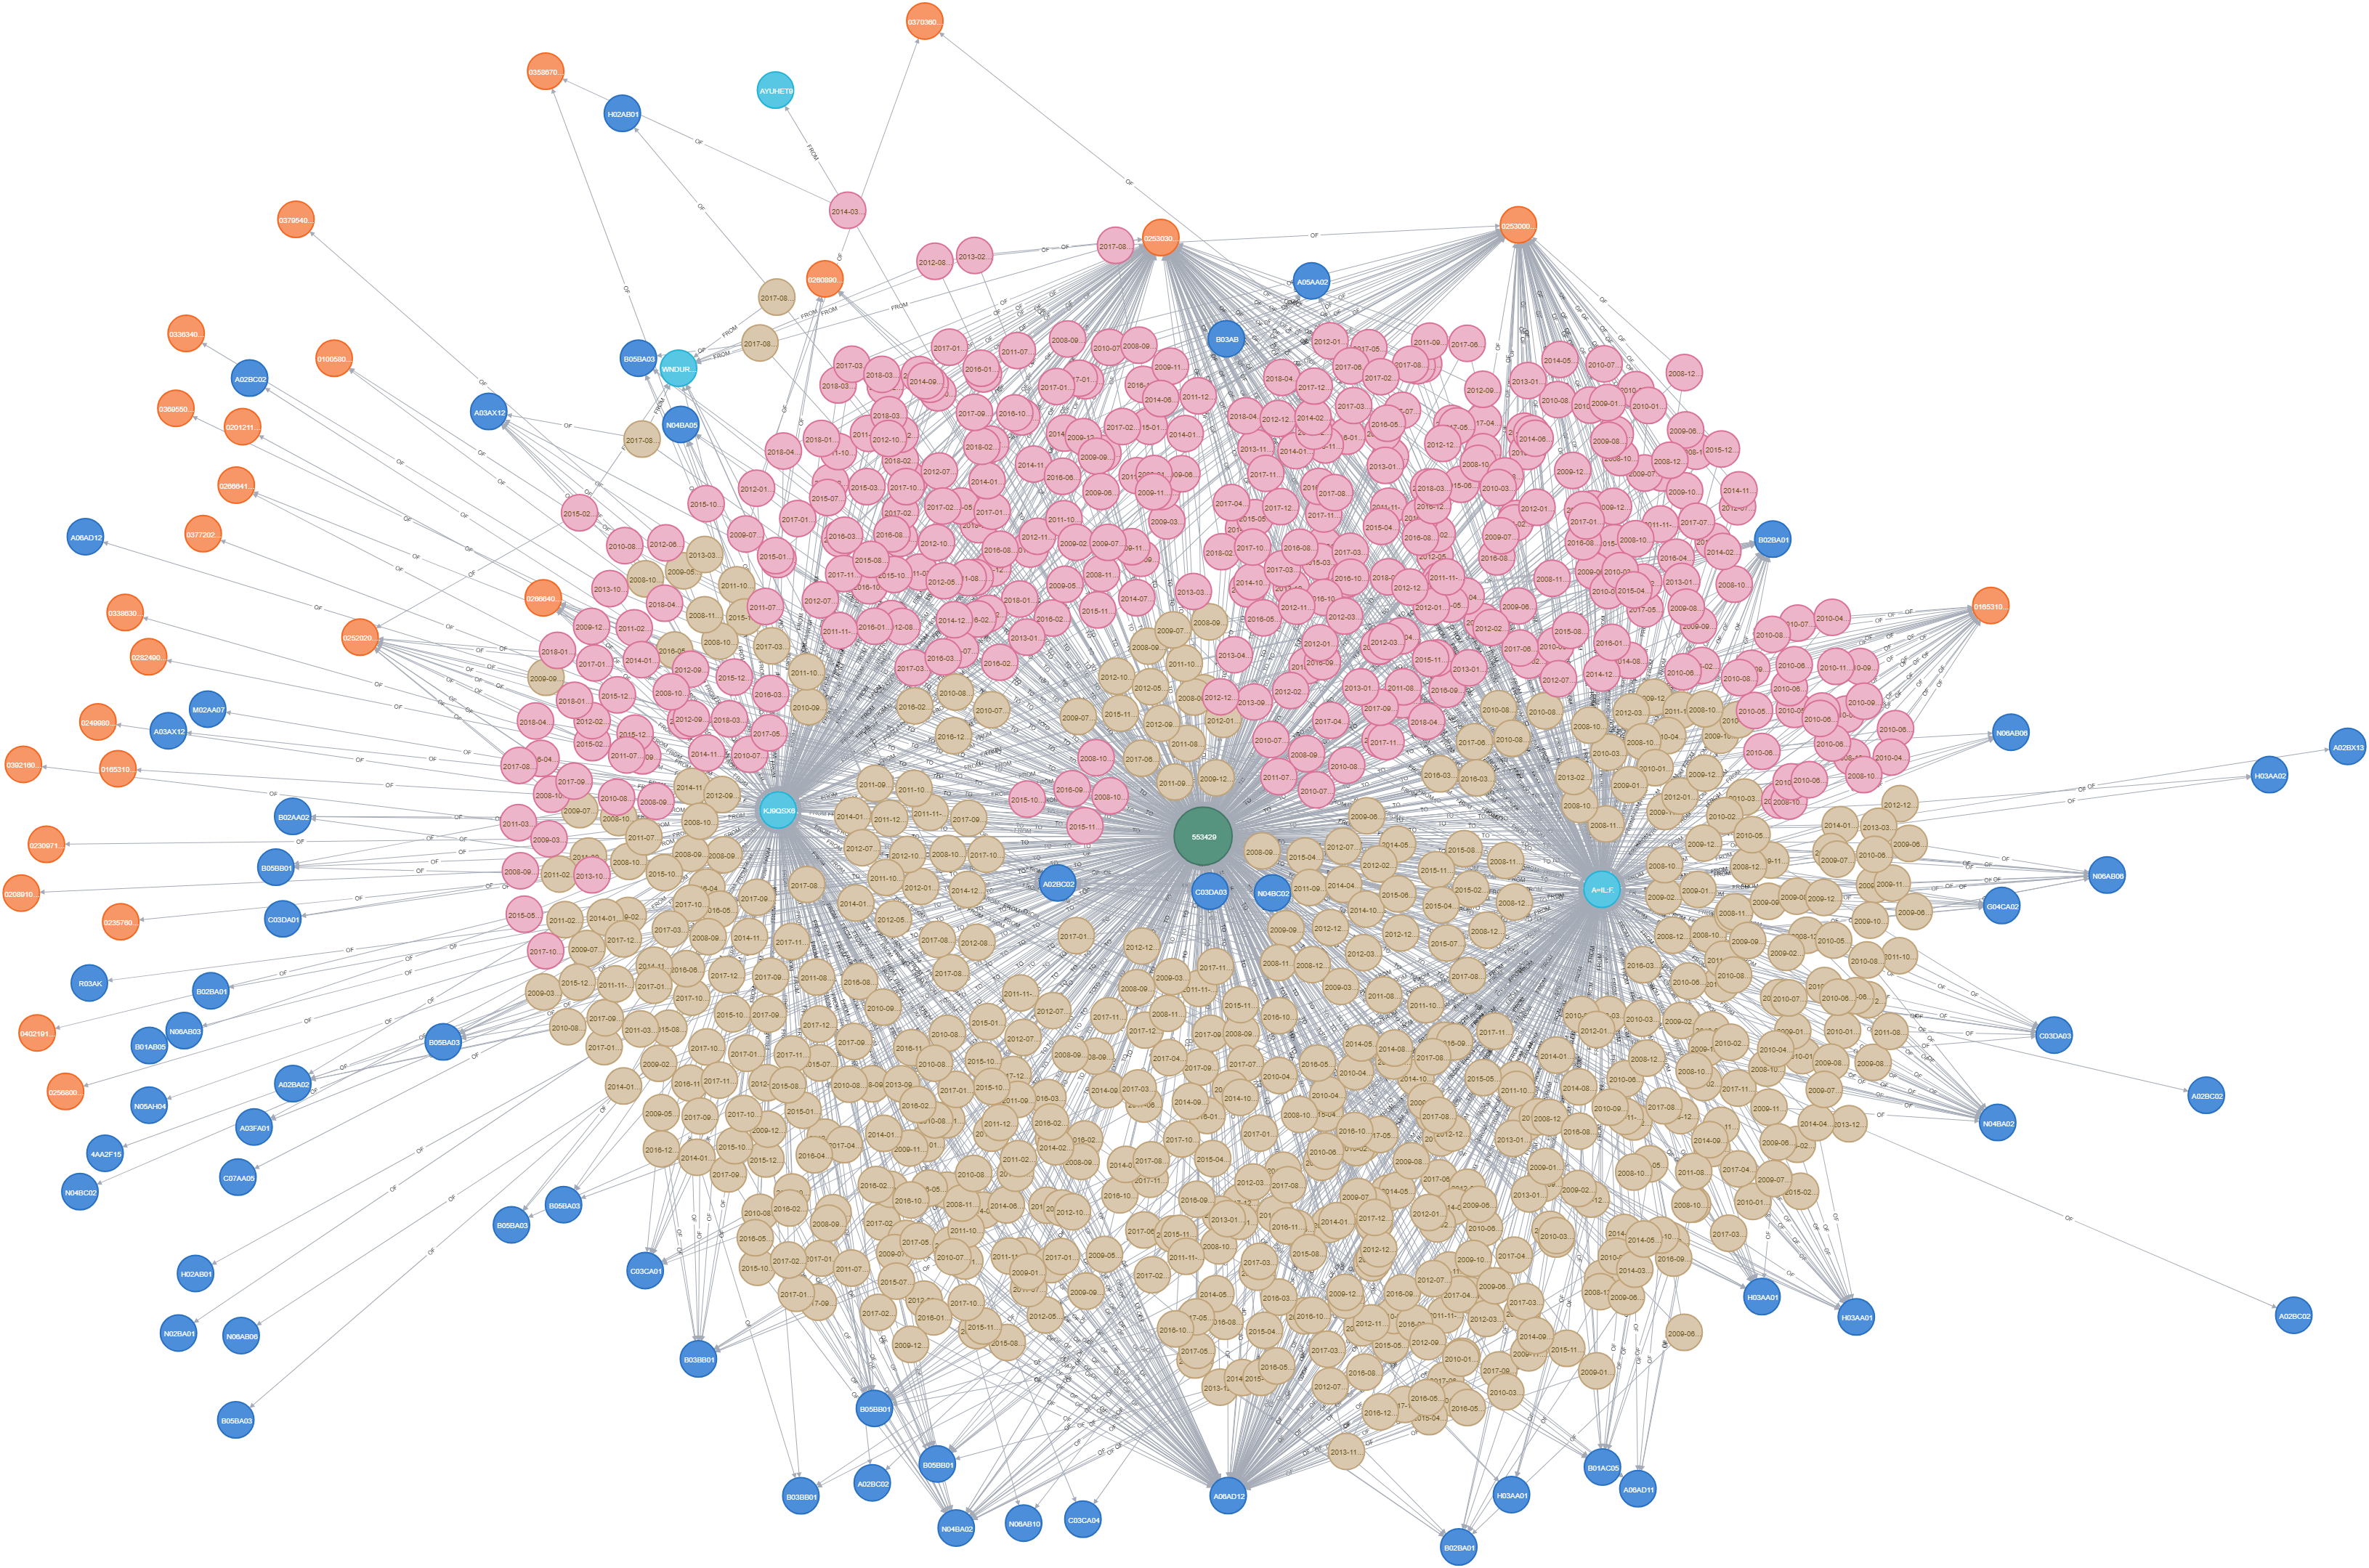
\includegraphics[scale=0.135]{./images/patient.png}
\end{figure}

Having a view focussed on prescriptions, the same procedure is applied extracting the 500th antibiotic in descending order according to number of prescriptions, corresponding to Locabiotal spray bottle 15 ml (50 mg / 5 ml).

The graph displays:
\begin{enumerate}
	\item 1 antibiotic, the orange node in the middle;
	\item 896 antibiotic prescriptions, the pink nodes;
	\item 107 doctors, the light blue nodes;
	\item 817 patients, the green nodes.
\end{enumerate}

\begin{figure}[h]
	\centering
	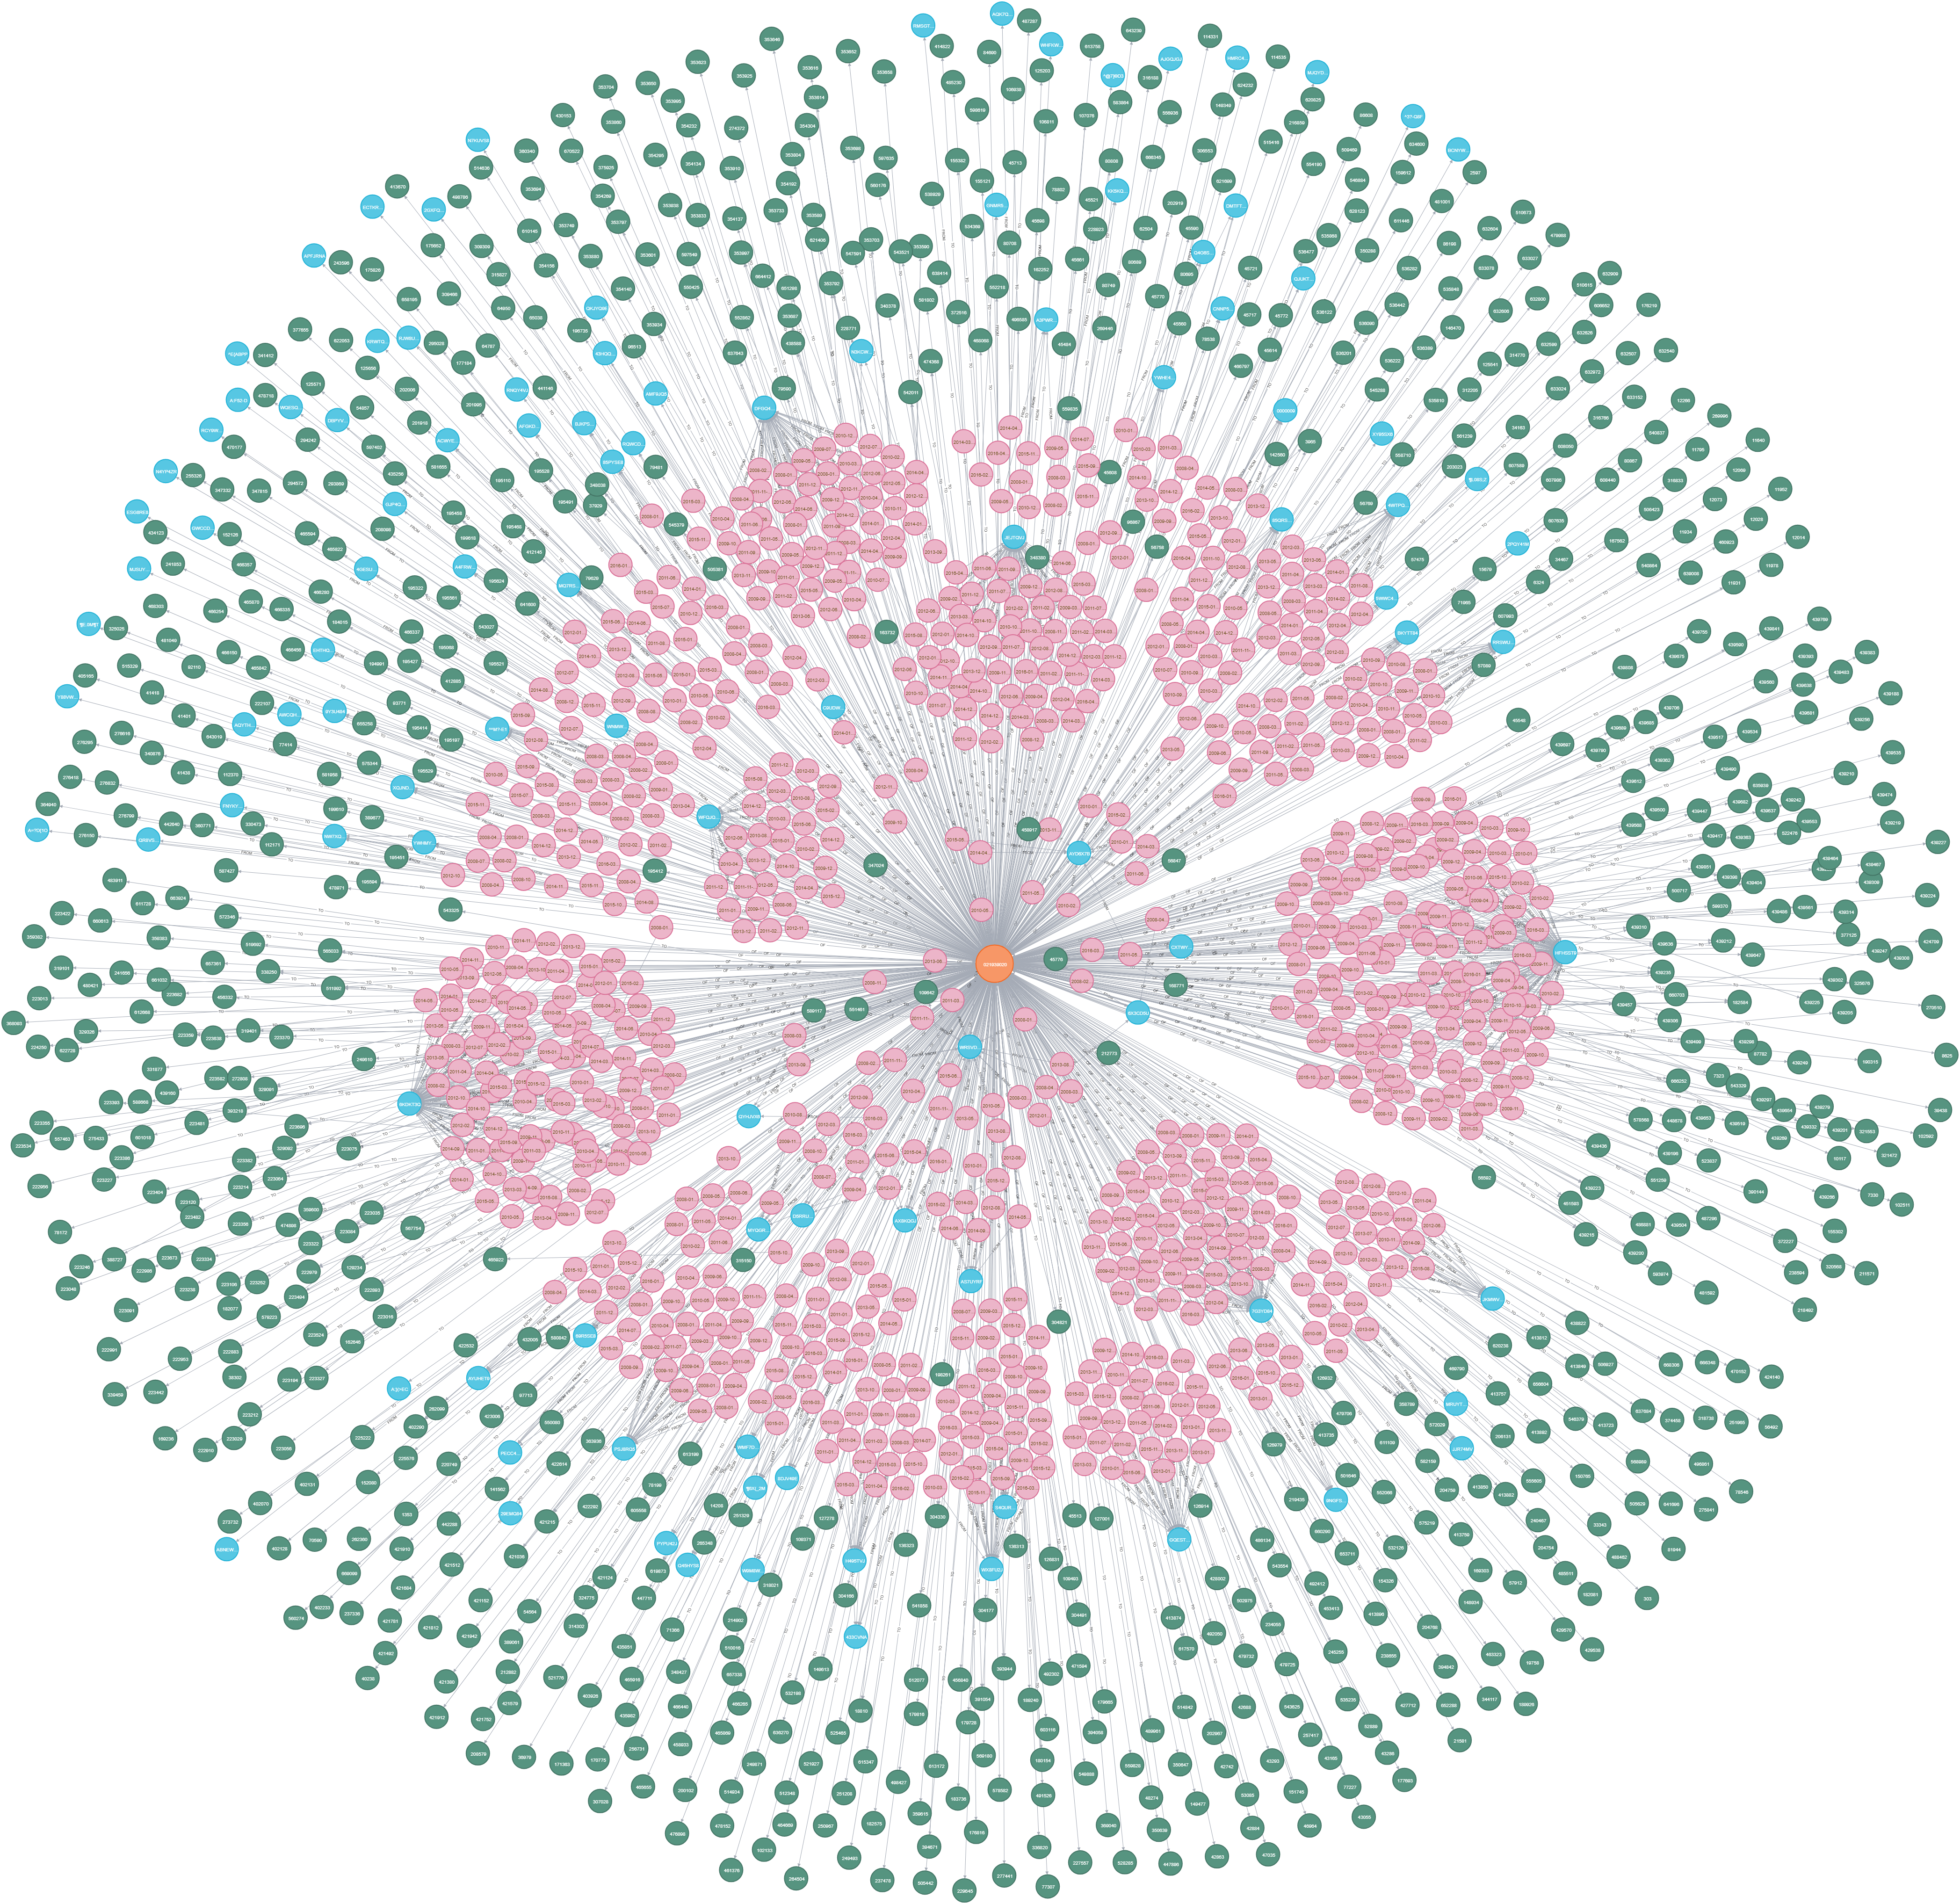
\includegraphics[scale=0.11]{./images/antibiotic.png}
\end{figure}

Those two examples allow to have a general idea of how nodes interact with each other, grouping in clusters. 

\subsection{Graph statistics}
A first set of global and local statistics are used to get the first insight on the graph and its components.

\begin{center}
	\begin{tabular}{c|c}
		Number of nodes & 16 611 005 \\
		\hline
		Number of relationships & 47 745 841 \\
		\hline
		Average prescriptions per doctor & 11 557,93 \\
		\hline
		Standard deviation & 15 457,6 \\
		\hline
		Maximum per doctor & 96 841 \\
		\hline
		Minimum per doctor & 1 \\
		\hline
		Average prescriptions per patient & 23,73 \\
		\hline
		Standard deviation & 40,46 \\
		\hline
		Maximum per patient & 1 567 \\
		\hline
		Minimum per patient & 1
	\end{tabular}
\end{center}

\subsection{Projecting a co-prescription graph}
Since the restriction on generic prescriptions involves having the same date and patient of another antibiotic prescription, couples are analysed adding a relationship between Antibiotic and Medicines in the main graph.

After counting the number of repetitions for each couple Antibiotic-Medicine, the first 100 most popular ones are used to couple nodes, with the amount as property of the relationship PRESCRIBED\_WITH.

Visualising the newly created relationships, two connected components are highlighted (orange antibiotics, blue other medicines).

\begin{figure}[h]
	\centering
	\includegraphics[scale=0.4]{./images/couples-graph.png}
\end{figure}

The component with only one couple corresponds to Plaquenil - Deltacortene, prescribed together approximately 5 000 times. Plaquenil can be used as antibiotic (antimalarial), but it is mostly given to treat arthritis, while Deltacortene is a corticosteroid for rheumatisms. 

The range of values varies from 4 145 to 38 153 in the timespan of 10 years. The 5 most popular co-prescriptions are:
\begin{enumerate}
	\item Augmentin - Oki;
	\item Rocefin - Bentelan;
	\item Augmentin - Bentelan;
	\item Normix - Cardioaspirin;
	\item Augmentin - Aulin.
\end{enumerate}

Bentelan is a corticosteroid which cannot be used without an antibiotic in presence of systemic (concerning the whole organism) infections\cite{bentelan}, since it is an immunosuppressive drug, and this would explain the frequent co-prescriptions.

All the antibiotics are among the most prescribed ones, which justifies their presence in the co-prescriptions as well.

\subsection{Projecting prescriptive habits}
Having a detailed view of doctors' most common prescriptions gives another insight on how antibiotics are related.

The three most prescribed antibiotics for each doctor are taken, along with their count, and a new relationship OFTEN\_PRESCRIBED between Doctor and Antibiotic is created. Only amounts of prescriptions greater or equal to 50 are taken into account, for consistency of results, resulting in 2 353 links.

The obtained graph displays:
\begin{enumerate}
	\item 809 doctors, the light blue nodes;
	\item 95 antibiotics, the orange nodes.
\end{enumerate}

\begin{figure}[h]
	\centering
	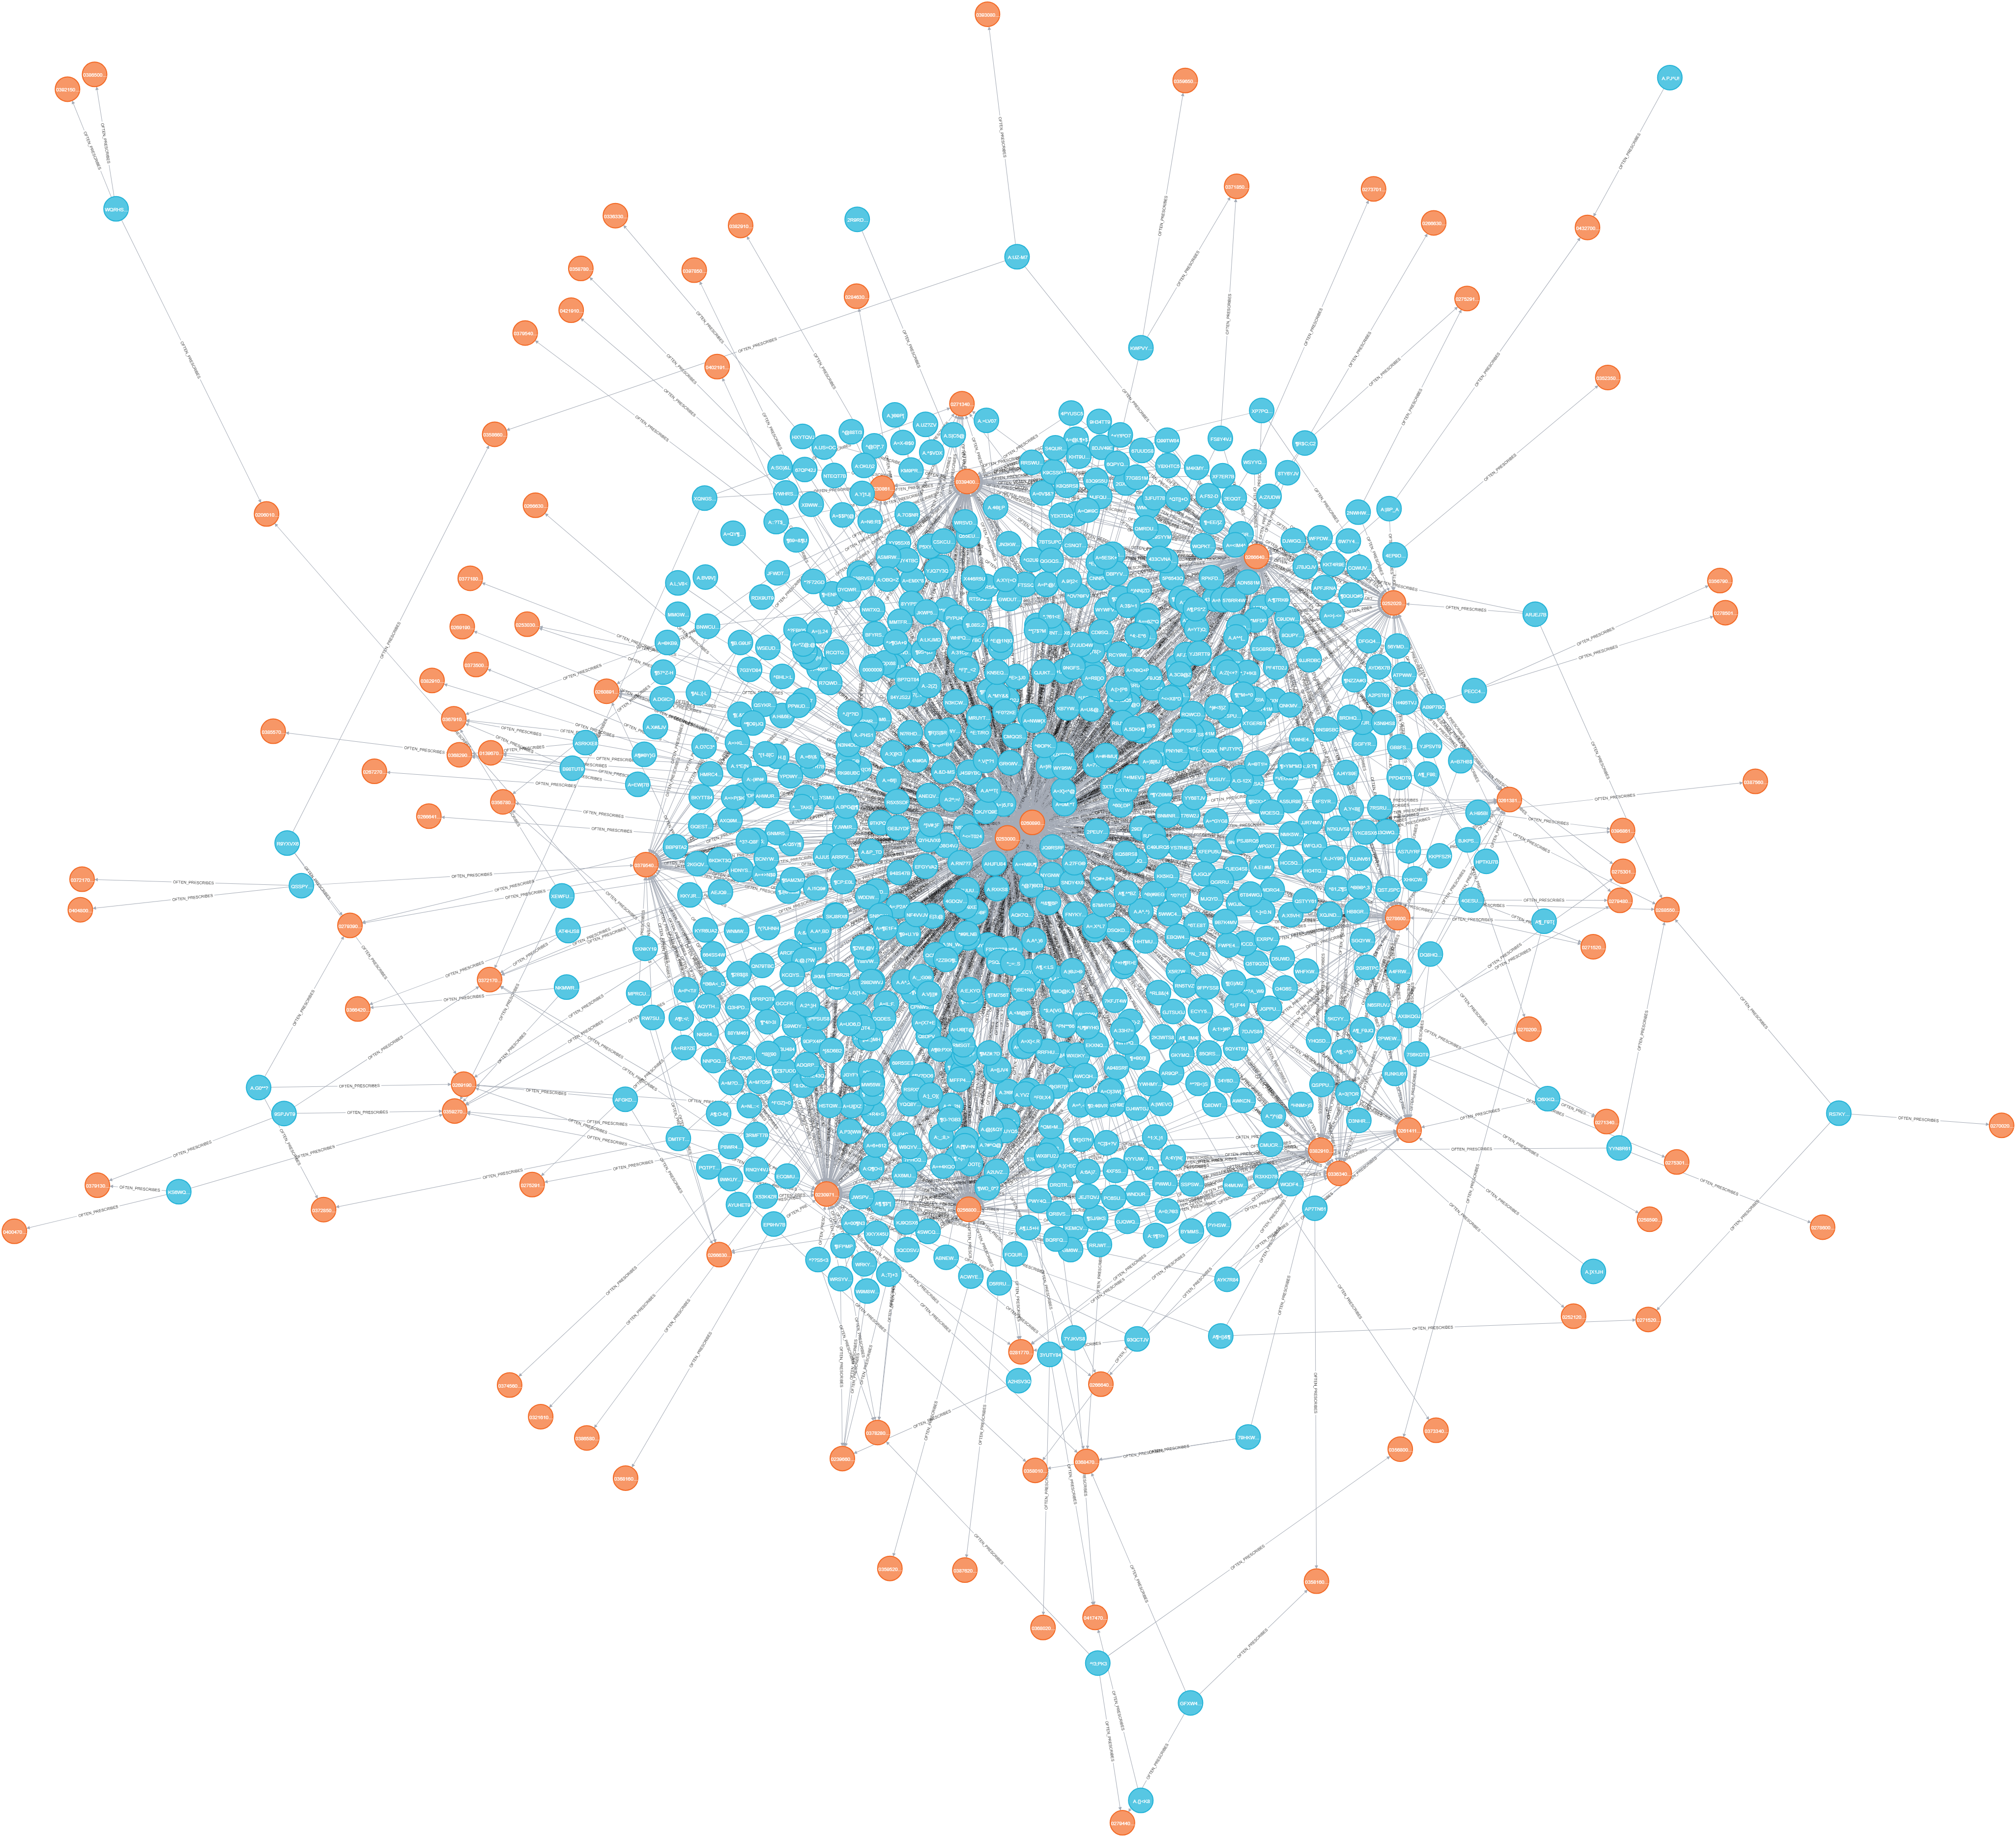
\includegraphics[scale=0.11]{./images/doctors-antibiotics-graph.png}
\end{figure}

Comparing the quantity of antibiotics and doctors and their relationships, it can be seen that most doctors prescribe a very restricted set of antibiotics.

To have a better understanding of the popularity of specific drugs, an auxiliary relationship PRESCRIBED\_BY\_SAME\_DOCTOR is created between Antibiotics. 

Antibiotics are interlinked with 294 new relationships:

\begin{figure}[h]
	\centering
	\includegraphics[scale=0.3]{./images/antibiotics-graph.png}
\end{figure}

\subsection{Centrality algorithms}

\subsubsection{Betweenness}
The Betweenness Centrality algorithm calculates the shortest (weighted) path between every pair of nodes in a connected graph, using the breadth-first search algorithm. 

Each node receives a score, based on the number of these shortest paths that pass through the node. Nodes that most frequently lie on these shortest paths will have a higher betweenness centrality score. 

Betweenness among the top 5 antibiotics:
\begin{center}
	\begin{tabular}{c|c}
		Antibiotic & Centrality \\
		\hline
		Augmentin (tablets) & 2 562 \\
		\hline
		Normix & 1 852, 74 \\
		\hline
		Velamox & 683, 78 \\
		\hline
		Ciproxin & 562, 71 \\
		\hline
		Augmentin (bottles) & 489,93 \\
	\end{tabular}
\end{center}

\subsubsection{Degree}
Degree Centrality is the simplest of all the centrality algorithms. It measures the number of incoming and outgoing relationships from a node, analysing its influence.

Degree among the top 5 antibiotics, according to co-prescriptions:
\begin{center}
	\begin{tabular}{c|c}
		Antibiotic & Degree \\
		\hline
		Augmentin (tablets) & 32 \\
		\hline
		Normix & 22 \\
		\hline
		Ciproxin & 14 \\
		\hline
		Augmentin (bottles) & 12 \\
		\hline
		Velamox & 10 \\
	\end{tabular}
\end{center}

Calculating degree among doctors is useful to determine whether the top antibiotics prescribers are also the top prescribers, using the top 5 doctors.

\begin{center}
	\begin{tabular}{c|c|c|c|c}
		Doctor & Degree (antibiotics) & Degree (medicine) & Total degree & Patients \\
		\hline
		1 & 45 625 & 51 221 & 96 846 & 4 466 \\
		\hline
		2 & 42 554 & 41 594 & 84 148 & 2 022 \\
		\hline
		3 & 35 645 & 22 383 & 58 028 & 1 816 \\
		\hline
		4 & 34 587 & 40 315 & 74 902 & 2 028 \\
		\hline
		5 & 34 380 & 28 763 & 63 143 & 1 874
	\end{tabular}
\end{center}

Seeing the obtained results, the overprescribing of some general practitioners is clear: most of them makes a number of antibiotic prescriptions equal to others having double the amount of patients.

Doctors prescribing too much and not strictly when needed is one of the main causes of antibiotic resistance in Italy.

% todo closeness?

\subsection{Community detection}
% cos'è la CD e perché

Communities are identified according to patients getting the same antibiotic or other medicine. To ease computational time, a new relationship GETS is created, with an attribute representing the number of time a patient received that determined prescription.

 \begin{wrapfigure}{L}{0.4\textwidth}
	\vspace{-10pt}
	\includegraphics[width=0.4\textwidth]{./images/patient-gets-graph.png}
	\vspace{-30pt}
\end{wrapfigure}

Since data is in the magnitude order of millions, only the top 10 most frequent antibiotics and medicines are selected, creating roughly 2 millions of relationships between 580 282 patients and 20 total drugs.

This means 85,5\% of patients received a prescription among a subset representing 0,08\% of antibiotics and other medicines.

\subsection{Similarity detection}


\section{Considerations}







 % seconda metà
\chapter{Assessments of results and future directions} % tutto
\begin{thebibliography}{}
	\footnotesize
	
	\bibitem{4vs}
	\texttt{https://healthitanalytics.com/news/understanding-the-many-vs-of-healthcare-big-data-analytics}
	
	\bibitem{millewin}
	\texttt{https://www.millewin.it/}
	
	\bibitem{generico}
	\texttt{https://www.normattiva.it/uri-res/N2Ls?urn:nir:stato:legge:1995-12-29;549~art3!vig=}
	
	\bibitem{aifaar}
	\texttt{http://www.agenziafarmaco.gov.it/content/la-resistenza-agli-antibiotici-emergenza-mondiale-il-primo-rapporto-globale-del-who}
	
	\bibitem{DC}
	Davide Castaldi, \textit{Richiesta Dati CNCM per Analisi Appropriatezza Prescrittiva}, Consorzio Milano Ricerche, 2018.
	
	\bibitem{draw}
	Made with \texttt{draw.io}.
	
	\bibitem{icd9}
	Manuale ICD-9-CM versione italiana 2007. \\
	\texttt{http://www.salute.gov.it/portale/documentazione/p6\_2\_2\_1.jsp?lingua=italiano\&id=2251}
	
	\bibitem{DC2}
	Davide Castaldi, \textit{Allegato Tech DB Campania}, Consorzio Milano Ricerche, 2018.
	
	\bibitem{atc}
	\texttt{https://bioportal.bioontology.org/ontologies/ATC} 
	
	\bibitem{medicinaliequivalenti}
	\texttt{http://www.agenziafarmaco.gov.it/sites/default/files/medicinali\_equivalenti-qualita\_sicurezza\_efficacia.pdf}
	
	\bibitem{aifa2017}
	\texttt{http://www.aifa.gov.it/sites/default/files/Rapporto-L'uso\_degli\_antibiotici\_in\_Italia\_2017\_0.pdf}
	
	\bibitem{dataquality}
	\texttt{http://mitiq.mit.edu/iciq/Documents/IQ\%20Conference\%201996/Papers/TheHealthCareIndustryandDataQuality.pdf}
	
	\bibitem{ehealth}
	\texttt{https://www.ncbi.nlm.nih.gov/pmc/articles/PMC1550636/}
	
	\bibitem{wonca2}
	\texttt{https://www.woncaeurope.org/sites/default/files/documents/Definizione\%20WONCA\%202011\%20ita\_A4.pdf}
	
	\bibitem{pg}
	\texttt{https://www.postgresql.org/}
	
	\bibitem{neo}
	\texttt{https://neo4j.com/}
	
	\bibitem{r}
	\texttt{https://www.r-project.org/}
	
	\bibitem{who}
	\texttt{https://www.who.int/en/news-room/fact-sheets/detail/antimicrobial-resistance}
	
	\bibitem{cdc}
	\texttt{https://www.cdc.gov/drugresistance/about.html}
	
	\bibitem{sweden}
	\texttt{https://www.folkhalsomyndigheten.se/contentassets/dae82c7afd424a57b57ec81818793346/swedish-work-on-containment-of-antibiotic-resistance.pdf}
	
	\bibitem{bmj}
	\texttt{bmj.com/cgi/pmidlookup?view=long\&pmid=9270458}
	
	\bibitem{oxford}
	\texttt{https://en.oxforddictionaries.com/definition/subsidiarity}
	
	\bibitem{ticket}
	\texttt{http://www.salute.gov.it/portale/esenzioni/dettaglioContenutiEsenzioni.jsp?lingua=italiano\&id=4674\&area=esenzioni\&menu=vuoto}
	
	\bibitem{classi}
	\texttt{http://www.fcr.re.it/classificazione-dei-farmaci-ai-fini-della-rimborsabilita}
	
	\bibitem{ricette}
	\texttt{https://web.archive.org/web/20111129162006/http://www.farmaciadicello.it/ricetta-01.htm}
	
	\bibitem{wonca1}
	\texttt{https://web.archive.org/web/20140611065109/http://www.woncaeurope.org/sites/default/files/documents/Definition\%203rd\%20ed\%202011\%20with\%20revised\%20wonca\%20tree.pdf}
	
	\bibitem{gp}
	\texttt{http://www.salute.gov.it/portale/temi/p2\_6.jsp?lingua=italiano\&id=1698\&area=tumori\&menu=percorso}
	
	\bibitem{ascpt}
	\texttt{https://ascpt.onlinelibrary.wiley.com/doi/full/10.1038/clpt.2008.24}
	
	\bibitem{whoicd}
	\texttt{https://www.who.int/classifications/icd/en/}
	
	\bibitem{icdit}
	\texttt{http://www.salute.gov.it/portale/temi/p2\_6.jsp?lingua=italiano\&id=1982\&area=statisticheSSN\&menu=definizioni}
	
	\bibitem{icd9en}
	\texttt{https://www.medicalbillingandcodingonline.com/icd-cm-codes/}
	
	\bibitem{aicdef}
	\texttt{http://www.agenziafarmaco.gov.it/glossary/term/1432}
	
	\bibitem{aic}
	\texttt{http://www.agenziafarmaco.gov.it/content/l\%E2\%80\%99autorizzazione-all\%E2\%80\%99immissione-commercio}
	
	\bibitem{atclevels}
	\texttt{https://www.whocc.no/filearchive/publications/2019\_guidelines\_web.pdf}
	
	\bibitem{repubblica}
	\texttt{https://www.repubblica.it/salute/medicina-e-ricerca/2019/03/13/news/antibioticoresistenza\_in\_italia\_il\_primato\_europeo\_di\_decessi-221467306/}
	
	\bibitem{antibiotic}
	\texttt{https://www.medicalnewstoday.com/articles/10278.php}
	
	\bibitem{calo}
	\texttt{https://www.aboutpharma.com/blog/2019/01/10/antibiotici-continua-il-calo-della-ricerca-e-sviluppo-secondo-locse/}
	
	\bibitem{usa}
	\texttt{https://clincalc.com/DrugStats/Top300Drugs.aspx}
	
	\bibitem{bacteria}
	\texttt{https://www.infectioncontroltoday.com/antibiotics-antimicrobials/study-shows-antibiotics-destroy-immune-cells-and-worsen-oral-infection}
	
	\bibitem{dedalus}
	\texttt{https://www.dedalus.eu/}
	
	\bibitem{datapine}
	\texttt{https://www.datapine.com/blog/big-data-examples-in-healthcare/}
	
	\bibitem{bentelan}
	\texttt{https://www.my-personaltrainer.it/Foglietti-illustrativi/Bentelan.html}
	
	\bibitem{agenziafarmaco}
	\texttt{http://www.agenziafarmaco.gov.it/content/la-resistenza-agli-antibiotici-emergenza-mondiale-il-primo-rapporto-globale-del-who}
	
	\bibitem{funnel}
	\texttt{https://www.fusioncharts.com/resources/chart-primers/funnel-chart}
	
\end{thebibliography}
	 % sistemare link

% entro 7 giugno: introduzione, pj
% entro 16 giugno (mariani): kmeans, results

\end{document}